\documentclass[12pt]{article}

\usepackage{ amsmath, amssymb, graphicx, psfrag, bm }
\usepackage[most]{tcolorbox}
\usepackage{amsmath,amsthm,amssymb}
\usepackage{mathtools}
\usepackage{listings}
\graphicspath{ {./images/} }

\addtolength{\textheight}{2.1in}
\addtolength{\topmargin}{-1.25in}
\addtolength{\textwidth}{2.03in}
\addtolength{\oddsidemargin}{-1.1in}
\addtolength{\evensidemargin}{-1.1in}
\setlength{\parskip}{0.1in}
\setlength{\parindent}{0.0in}

\pagestyle{plain}

\raggedbottom
 
\newcommand{\given}{\, | \,}
\newcommand{\lrp}[1]{\left(#1\right)}
\newcommand{\lrb}[1]{\left[#1\right]}
\newcommand{\lrc}[1]{\left\{#1\right\}}
\newenvironment{solution}{\begin{tcolorbox}[breakable]\begin{proof}[\textbf{\textit{Solution}}] }{\end{proof}\end{tcolorbox}}
\newcommand{\bi}[1]{\textbf{\textit{#1}}}
\renewcommand\labelitemi{$\blacktriangleright$}
\newcommand{\bb}{\mathcal{B}}
\newcommand{\btheta}{\bm{\theta}}
\newcommand{\by}{\bm{y}}
\newcommand{\tcr}[1]{\textcolor{red}{#1}}
\renewcommand\labelitemi{$\blacktriangleright$}
 
\begin{document}

\begin{flushleft}

Prof.~David Draper \\
Department of Statistics \\
Baskin School of Engineering \\
University of California, Santa Cruz \\
Winter 2022

\end{flushleft}

\Large

\begin{center}

STAT 206 (\textsf{Applied Bayesian Statistics})

\fbox{\textbf{Take-Home Test 3: Part 2 (\textit{Revised} 17 Mar 2022)}}

\large

\textbf{Absolute due date}: uploaded to \texttt{canvas.ucsc.edu} by 11.59pm on \textbf{20 Mar 2022}

\end{center}


\normalsize
\textbf{Name:} Kevin Guillen


Here are the \bi{revised} ground rules: this test is open-book and open-notes, and has three parts. Part 1 consists of 7 true/false questions, each worth 10 points, for a total of 70 points; this part is \bi{mandatory for all STAT 206 students}. Part 2 has a single calculation question in it, worth 220 points; this part is also \bi{mandatory for all STAT 206 students}. Part 3 is entirely \bi{optional for all STAT 206 students} and acts as a source of \bi{extra credit} (up to 220 additional points): any points earned here will be added to the numerator, but not the denominator, in computing your course percentage correct 

\hspace*{0.5in}\bi{( total points achieved ) / ( total points assigned )} .

Undergraduates who wish to gain full mastery of all of the material presented this quarter are strongly encouraged to participate in office hour sessions from now through Sun 20 Mar 2022.

Some advice on style as you write up your solutions: pretend that you're sitting next to the grader, having a conversation about problem $( x )$ part $( y )$. You say, ``The answer is $z$,'' and the grader says, ``Why?'' You then give your explanation, as succinctly as possible to get your idea across. The right answer with no reasoning to support it, or incorrect reasoning, will get \textbf{half credit}, so try to make a serious effort on each part of each problem (this will ensure you at least half credit). In an AMS graduate class I taught in 2012, on a take-home test like this one there were 15 true/false questions, worth a total of 150 points; one student got a score of 92 out of 150 (61\%, a D$-$, in a graduate class where B$-$ is the lowest passing grade) on that part of the test, for repeatedly answering just ``true" or ``false" with no explanation. Don't let that happen to you.  

On each problem, the graders and I mentally start everybody out at $-0$ (i.e., with a perfect score), and then you accumulate negative points for incorrect answers and/or reasoning, or parts of problems left blank.

This test is to be entirely your own efforts; do not collaborate with
anyone or get help from anyone but me or our TA (Jacob Fontana). The intent is that the course lecture notes and readings should be sufficient to provide you with all the guidance you need to solve the problems posed below, but you may use other written materials (e.g., the web, journal articles, and books other than those already mentioned in the readings),
\textbf{provided that you cite your sources thoroughly and accurately}; you
will lose (substantial) credit for, e.g., lifting blocks of text directly
from \texttt{wikipedia} and inserting them into your solutions without full
attribution.

If it's clear that (for example) two people have worked together on a part
of a problem that's worth 20 points, and each answer would have earned 16
points if it had not arisen from a collaboration, then each person will
receive 8 of the 16 points collectively earned (for a total score of 8 out
of 20), and I reserve the right to impose additional penalties at my
discretion. If you solve a problem on your own and then share your solution
with anyone else, you're just as guilty of illegal collaboration as
the person who took your solution from you, and both of you will receive
the same penalty. This sort of thing is necessary on behalf of the many
people who do not cheat, to ensure that their scores are meaningfully
earned. In the AMS graduate class in 2012 mentioned above, five people failed the class because of illegal collaboration; don't let that happen to you.

In class I've demonstrated numerical work in \texttt{R}; you can (of course) make the calculations and plots requested in the problems below in any environment you prefer (e.g., \texttt{Matlab}, ...). To avoid plagiarism, if you end up using any of the code I post on the course web page or generate during office hours, at the beginning of your Appendix (see below) you can say something like the following: \vspace*{-0.1in} 

\begin{quote}

\bi{I used some of Prof.~Draper's \texttt{R} code in this assignment, adapting it as needed.} \vspace*{-0.25in} 

\end{quote}

Those of You who are using \texttt{LaTeX} or some other word-processing environment to prepare Your solutions can stick quote blocks below each question, into which You can type Your answers (I suggest that You use \textbf{bold} or \textit{italic} font to distinguish Your solutions from the questions). If You're submitting Your answers in longhand, which is perfectly acceptable, You can just write them out on separate sheets of paper, making sure that the grader can easily figure out which chunk of text is the solution to which part of which problem.
\begin{quote}

\bi{Please collect \{all of the code you used in answering the questions  below\} into an Appendix at the end of your document, so that (if you do something wrong) the grader can more accurately give you part credit.} 

\end{quote}

Parts 2 and 3 of this test are similar to problem 2(B) in Take-Home Test 2, in that they look really long but don't actually have that much for You to do: just read the problems carefully, run my code (sometimes You'll need to modify it a bit), and figure how to interpret the output.

\section*{Part 2:~Calculation}

\bi{[220 total points for this problem]} As I'm sure You know, if You encounter a wild mushroom in a forest there's no guarantee that it's edible; every year several people die in the U.S.~from wild mushroom poisoning. Two questions come to mind, in this age of cell phone apps: (1) Can the edible/poisonous status of a wild mushroom be accurately predicted from characteristics such as its appearance and odor? and (2) If You were building an app to give people advice about whether a wild mushroom they've found is edible, (to make the app easy to use) what's the minimum number of variables necessary to get highly accurate predictions?

The \textit{U.C.~Irvine Machine Learning Repository} has a data set -- a copy of which is now available in the \texttt{Pages} tab of the course \texttt{Canvas} page, along with a text file containing important contextual information -- consisting of $n =$ 8,124 

\begin{quote}

hypothetical samples corresponding to 23 species of gilled mushrooms in the \textit{Agaricus} and \textit{Lepiota} Family. Each species is identified as
definitely edible, definitely poisonous, or of unknown edibility and not recommended. This latter class was combined with the poisonous one. The \textit{Audubon Society Field Guide to North American Mushrooms} (1981) clearly states that there is no simple rule for determining the edibility of a mushroom; no rule like ``leaflets three, let it be'' for Poisonous Oak and Ivy.

\end{quote}

As You'll see when You begin looking at the data set, there are $k = 22$ predictor variables $( x_1, \dots, x_k )$ available, ranging from aspects of the mushroom's cap to its habitat, and the outcome variable $y$ is coded 1 for poisonous and 0 for edible. The goals of this problem, corresponding to the two questions above, are (1) to build linear regression models, using these predictors, to produce estimated probabilities $\hat{ p }$ that $( y = 1 )$ as a function of a given mushroom's characteristics, (2) to identify the smallest subset of the $x_j$ (for inclusion in the app) that still produces highly accurate $\hat{ p }$ values, and (3) to decide whether the predictive modeling in step (2) is accurate enough to release the app to the general public without poisoning a lot of people in the process.

We're going to do a maximum-likelihood analysis of this data set, because (I'm assuming that) You and I know so little about `gilled mushrooms in the \textit{Agaricus} and \textit{Lepiota} Family' that a Bayesian analysis here would just reproduce the likelihood story. I'm also doing something a bit unusual in having You fit \textit{linear} regression models to a binary outcome variable, but the more usual choice of \textit{logistic} regression models (like those in part 3 of this test) would give essentially the same results.

When You examine the set of predictor variables, You'll see that they're all categorical (\texttt{R} calls such variables \textit{factors}), taking on a number of possible values (\textit{levels}) ranging from 1 to 12. 

\begin{quote}

\textbf{\fbox{\textit{Important:}} \vspace*{0.025in} All of the levels of all of the predictors in the data set have been abbreviated to a single letter in the standard English alphabet; the context file contains a dictionary that translates those abbreviations to their actual meanings.} 

\end{quote}

Obviously any predictor variable that takes on only 1 possible value is useless for predicting anything; there is such a variable, so early on in the analysis we'll drop it (\texttt{veil.type}) and reset $k$ to 21. One variable -- \texttt{stalk.root} -- has a lot of missing values (2,480 out of 8,124), but one nice thing about categorical predictors is that \textit{missingness can be treated as just another level of the factor}, so that no cases are lost by having to omit rows in the data set with missing values in them (that would be an undesirable action that's not needed with factor predictors). If those 2,480 values are \textit{Missing Completely At Random} (MCAR; see Quiz 2), this will just make 
\texttt{stalk.root} noisier as a predictor; if they're not MCAR, we can use the fact of their missingness in the prediction process\footnote{Ideally we should do a sensitivity analysis in which the 2,480 rows are temporarily omitted from the data set, to see if we get the same results as those that arise when those rows are included; I've decided not to ask You to do that here, because the problem is already fairly long.}.

As discussed in class, the basic frequentist (multiple) linear regression model is of the form (for $i = 1, \dots, n )$
\begin{equation} \label{e:linear-regression-1}
y_i = \beta_0 + \sum_{ j = 1 }^k x_{ ij } \, \beta_j + e_i \, ,
\end{equation}
in which the $( e_i \given \sigma \, [ SM \! \! : \! \mathbb{ N } ] \, \mathcal{ B } )$ are IID $N ( 0, \sigma^2 )$; here $[ SM \! \! : \! \mathbb{ N } ]$ denotes the Normality assumption for the sampling model (SM), which is not part of problem context. In class we also saw that this model can be written in matrix form as
\begin{equation} \label{e:linear-regression-2}
\bm{ y } = X \, \bm{ \beta } + \bm{ e } \, ,
\end{equation} 
where $\bm{ y }$ is the $( n \times 1 )$ column vector whose transpose is $( y_1, \dots, y_n )$, $X$ is the $[ n \times ( k + 1 ) ]$ matrix whose first column is a vector of 1s (to account for the intercept term $\beta_0$) and whose $i$th row is $( 1, x_{ i1 }, \dots, x_{ ik } )$, $\bm{ \beta }$ is the $[ ( k + 1 ) \times 1 ]$ column vector whose transpose is $( \beta_0, \beta_1, \dots, \beta_k )$ and $\bm{ e }$ is the $( n \times 1 )$ column vector whose transpose is $( e_1, \dots, e_n )$. 

In applying this model to the mushroom data, a new question immediately arises: how can You bring a categorical predictor -- such as the 18th predictor in the data set \texttt{ring.number}, with the 3 levels ``n'' (none), ``o'' (one) and ``t'' (two) -- into a regression model? The answer is with a set of \textit{indicator}, also known as \textit{dummy}, variables: with $x_{ \{ 18 \} }$ = \texttt{ring.number} as an example (here $x_{ \{ 18 \} }$ means the 18th predictor variable), having $\ell = 3$ levels, You create a new variable $z_1$ that's 1 if $x_{ \{ 18 \} } =$ ``n'' and 0 otherwise, and another new variable $z_2$ that's 1 if $x_{ \{ 18 \} } =$ ``o'' and 0 otherwise, and a third new variable $z_3$ that's 1 if $x_{ \{ 18 \} } =$ ``t'' and 0 otherwise. 

If You now include all $\ell = 3$ of the $z_j$ in the set of predictors, in place of $x_{ \{ 18 \} }$, You will have created what's called a \textit{collinearity} problem: by the nature of how the $z_j$ were defined, for every mushroom $i$ in the data set it's a fact that $z_{ i1 } + z_{ i2 } + z_{ i3 } = 1$. This makes the $X$ matrix in equation (\ref{e:linear-regression-2}) non-invertible, meaning that the computation of the maximum-likelihood estimate of $\bm{ \beta }$, namely $\hat{ \bm{ \beta } } = ( X^T X )^{ -1 } \, X^T \, \bm{ y }$, would be more difficult to carry out. The (simple) solution is to omit one of the $z$ variables in the set of $z_j$ You include in the modeling: after all, in the \texttt{ring.number} example, if You knew $z_{ i1 }$ and $z_{ i2 }$, $z_{ i3 } = ( 1 - z_{ i1 } - z_{ i2 } )$ would be redundant (in the jargon of regression modeling, the category whose $z$ dummy has been left out is called the \textit{omitted group}). Letting $\ell_j$ be the number of levels of categorical predictor $x_j$ and setting $L = \sum_{ j = 1 }^k \ell_j$, the new linear regression model, expressed in terms of the dummy variables $z$, is
\begin{eqnarray} \label{e:linear-regression-3}
y_i & = & \beta_0 + \left[ \beta_1 \, z_{ i1 } + \dots + \beta_{ \ell_1 - 1 } \, z_{ i, \ell_1 - 1 } \right] + \left[ \beta_{ \ell_1 } \, z_{ i2 } + \dots + \beta_{ \ell_1 + \ell_2 - 2 } \, z_{ i, \ell_1 + \ell_2 - 2 } \right] \\ \nonumber 
& & \hspace*{0.25in} + \dots + \left[ \beta_{ L - K - ( \ell_k - 2 ) } \, z_{ i, L - K - ( \ell_k - 2 ) } + \dots + \beta_{ L - k } \, z_{ i, L - k } \right] + e_i \, .
\end{eqnarray}
This looks nasty but isn't: original categorical variable (factor) $x_1$ is replaced by $( \ell_1 - 1 )$ dummy variables, original factor $x_2$ is replaced by $( \ell_2 - 1 )$ dummies, and so on up to original factor $x_k$ being replaced by $( \ell_k - 1 )$ dummies, for a total of $k^* = ( L - k )$ dummy variables replacing the original $k$ factors. In the mushroom data set there are  $k = 21$ non-trivial factors as predictor variables, and the total number of dummies needed to carry this information is $[ ( 6 + 4 + 10 + 2 + 9 + 2 + 2 + 2 + 12 + 2 + 5 + 4 + 4 + 9 + 9 + 4 + 3 + 5 + 9 + 6 + 7 ) - 21 ] = 95$. (Where did I get the numbers $( 6 + 4 + \dots + 7 )$?)

\begin{itemize}

\item[(a)]

\bi{[10 total points for this sub-problem]} Create a new directory for this case study and download into this directory all of the files in the Pages tab of the course Canvas page that have `mushroom' in their names. I've written some \texttt{R} code for You, to start You on the analysis of this data set; it's in the file you just downloaded called

\hspace*{1.0in} \texttt{stat-206-mushroom-data-analysis.txt}

There's a block of code at the top of the file that begins \texttt{`the first block of code starts here'} and ends \texttt{`the first block of code ends here'}; run this code block and study the output. The function \texttt{tab.sum} in this code block provides diagnostic information on whether a factor $x$ will turn out to be predictively useful in the modeling; briefly explain in what sense \texttt{tab.sum} provides such information (\textit{Hint:} the function estimates the conditional mean (and SD, not useful here) of what variable given what other variable?). \bi{[10 points]}

\begin{solution}
    Well from the data output we see the first column is the different cap shapes alongside their $n$, mean and SD. This is to tell us the conditional expectation of the mean based on poisonous or not at each level of the given factor. That is to really say it gives us the probability that given mushroom cap shape is poisonous
\end{solution}

\item[(b)]

\bi{[20 total points for this sub-problem]} Run the second code block, in which a linear regression model is fit with the dichotomous outcome \texttt{poisonous} regressed on the factor \texttt{cap.shape}, and study the output. When the predictions $\hat{ y }$ from equation (\ref{e:linear-regression-3}) are specialized to this regression, they looks like
\begin{equation} \label{e:linear-regression-4}
\hat{ y }_i = \hat{ \beta }_0 + \hat{ \beta }_1 \, z_{ i1 } + \dots + \hat{ \beta }_5 \, z_{ i5 } \, ,
\end{equation} 
in which the $\hat{ \beta }_j$ are the maximum-likelihood estimates of the regression coefficients and where \{$z_{ i1 } =$ 1 if \texttt{cap.shape} = `c' and 0 otherwise\}, \{$z_{ i2 } =$ 1 if \texttt{cap.shape} = `f' and 0 otherwise\}, and so on down to \{$z_{ i5 } =$ 1 if \texttt{cap.shape} = `x' and 0 otherwise\}. Now examine the extracts from the \texttt{tab.sum} and regression fitting in Table \ref{t:data-analysis-1}. Explicitly identify $( \hat{ \beta }_0, \dots, \hat{ \beta }_5 )$ in the output in the table \bi{[10 points]}, and -- by thinking about the form of equation (\ref{e:linear-regression-4}) for each of the levels of \texttt{cap.shape} -- explicitly relate the numbers in the \texttt{mean} column of the \texttt{tab.sum} output in Table \ref{t:data-analysis-1} to the $\hat{ \beta }_j$. \bi{[10 points]}

\begin{table}[t!]

\centering

\caption{\textit{Extracts from the output of the second code block.}}

\begin{verbatim}
          #      cap.shape n    mean      sd       

          # [1,] 1         452  0.1061947 0.308428 
          # [2,] 2         4    1         0        
          # [3,] 3         3152 0.4936548 0.5000391      output of tab.sum
          # [4,] 4         828  0.7246377 0.4469667
          # [5,] 5         32   0         0        
          # [6,] 6         3656 0.4671772 0.4989898

          # Coefficients:
          #             Estimate Std. Error t value Pr(>|t|)    
          # (Intercept)  0.10619    0.02279   4.659 3.22e-06 ***
          # cap.shapec   0.89381    0.24335   3.673 0.000241 ***   output of
          # cap.shapef   0.38746    0.02437  15.898  < 2e-16 ***   linear
          # cap.shapek   0.61844    0.02834  21.824  < 2e-16 ***   regression
          # cap.shapes  -0.10619    0.08864  -1.198 0.230926    
          # cap.shapex   0.36098    0.02416  14.942  < 2e-16 ***
\end{verbatim}

\label{t:data-analysis-1}

\end{table}

\begin{solution}
    It is clear from the table that we get our $\hat{\beta}_j$ value from the "Estimate" column on the table. So,
    \[(\hat{\beta_1}, \hat{\beta_2} , \dots, \hat{\beta_5}) = (0.10619, 0.89381, 0.38746 , 0.61844 , -0.10619 ,0.36098  ).\]

    We see that $\hat{\beta_0}$ is equal to the mean about "poisonous" when cap shape is "b". This follows from (4) by,
    \[\hat{y_b} = 0.10619 + \hat{\beta_1}0 + \dots + \hat{\beta_5}0 = 0.10619\]

    To see the way it relates to the rest of the mean values relate to the rest of $\hat{\beta_j}$ let's look at when cap.shape $='c'$,
    \begin{align*}
        \hat{y_c} = 0.10619 + 0.89381\cdot 1  + \hat{\beta_2}\cdot 0 + \dots + \hat{\beta_5}\cdot 0 = 1
    \end{align*}
    which matches the mean table for mushroom cap $f$. Which means the relation is,
    \[E(y \given \text{cap.shape} = i) = \bar{y_i} = \hat{y_i}.\]
    More directly in terms of $\hat{\beta}_j$ the relation it is that $\hat{\beta_0}$ is equal to the mean $y$ in the omitted category. Then for $j \geq 1$ we have $\hat{\beta_j}$ is equal to the mean $y$ in category $j$ minus the mean $y$ in the omitted category. 
\end{solution}

\item[(c)]

\bi{[40 total points for this sub-problem]} Toward the end of the second code block, the code computes predicted $\hat{ p } = P ( y = 1 \given x_1 \, [ SM \! \! : \! \mathbb{ L } ] \, \mathcal{ B } )$ values (in which $[ SM \! \! : \! \mathbb{ L } ]$ signifies the linear regression modeling assumption, which is not part of $\mathcal{ B }$), makes a diagnostic plot and computes a numerical diagnostic -- the \textit{Predictive Separation Index (PSI)} -- measuring the predictive strength of the factor \texttt{cap.shape}.

\begin{itemize}

\item[(i)]

\bi{[20 total points for this sub-problem]} The diagnostic plot is in two parts: the top panel is a histogram of the $\hat{ p }$ values for the mushrooms for which $y = 0$, and the bottom panel shows the same thing except for the cases in which $y = 1$. What would the ideal shape of these histograms be, if a factor $x$ offers perfect information for predicting a dichotomous outcome $y$? Explain briefly \bi{[10 points]}. Do the histograms achieve that goal with the predictor \texttt{cap.shape}? Explain briefly \bi{[10 points]}.

\begin{solution}
    For the histogram of $y = 0$, the ideal shape would be a single spike at 0, meaning all $\hat{p}$ equalling 0 and nothing else. For when $y = 1$, the ideal shape would be a single spike at 1, meaning all the $\hat{p}$ equalling 1 and nothing else. This is because this would mean they are perfect predictions since our true value for the histograms is either $y = 0 $ or $1$, without loss of generality, if $y = 1$ ideally we would want to have perfect prediction, meaning all the $\hat{p} = 1$ since that is the truth.  

    Knowing these ideal histograms and comparing, we see cap.shape is a horrible predictor. This is because we see for both graphs most the spikes are concentrated at around 0.48, far away from what we ideally want. 
\end{solution}

\item[(ii)]

\bi{[20 total points for this sub-problem]} The PSI, which is a numerical index that goes hand-in-hand with the diagnostic plot, is defined as follows:
\begin{equation} \label{e:psi-1}
PSI ( x ) = [ \textrm{mean } ( \hat{ p } \textrm{ given } x ) \textrm{ when } y = 1 ] - [ \textrm{mean } ( \hat{ p } \textrm{ given } x ) \textrm{ when } y = 0 ] \, .
\end{equation}
What's the ideal value of the $PSI$, if a factor $x$ is perfectly predictive of $y$? Explain briefly \bi{[10 points]}. Does the $PSI$ come close to achieving that goal with \texttt{cap.shape}? Explain briefly \bi{[10 points]}.

\begin{solution}
    Well recall what we said in the last part. If our histograms were ideal it would mean when $y = 1$ all our $\hat{p}$ values would be equal to 1 and if $y = 0$ then all our $\hat{p}$ values would be equal to 0. So if we were to take the mean of all the $\hat{p}$ in the ideal case when $y = 1$, then the mean should also be 1. Similarly the mean of all the $\hat{p}$ in the ideal case when $y = 0$ should be 0. Therefore when calculating the $PSI$ in the ideal case we would get $PSI(x) = 1 - 0 = 1$. We see though after running the code provided we get, 
    \[PSI(x) =0.51326496 -  0.45295970  =  0.06030526\]
    Which we see is ridiculously far from ideal, meaning we don't come close to achieving our goal $PSI$ with cap.shape.
\end{solution}

\end{itemize}

\begin{table}[t!]

\centering

\caption{\textit{Predictive accuracy of each of the factors $x$ in the mushroom data set, with $PSI$ sorted from largest to smallest.}}

\bigskip

\begin{tabular}{c|cc}

Factor $( x )$ & $PSI$ & Predictive Power \\

\hline

\texttt{odor} & 0.942 & extremely strong \\ 

\texttt{spore.print.color} & 0.566 & strong \\ 

\texttt{gill.color} & 0.464 & moderate \\

\texttt{ring.type} & 0.363 & moderate \\ 

\texttt{stalk.surface.above.ring} & 0.346 & moderate \\ 

\texttt{stalk.surface.below.ring} & 0.3304 & moderate \\ 

\texttt{gill.size} & 0.292 & moderate \\

\texttt{stalk.color.above.ring} & 0.275 & moderate \\

\texttt{stalk.color.below.ring} & 0.265 & moderate \\

\texttt{bruises} & 0.252 & moderate \\

\texttt{population} & 0.238 & weak \\ 

\texttt{habitat} & 0.194 & weak \\

\texttt{stalk.root} & 0.165 & weak \\

\texttt{gill.spacing} & 0.121 & weak \\

\texttt{cap.shape} & 0.0603 & weak \\

\texttt{cap.color} & 0.0477 & weak \\

\texttt{ring.number} & 0.0461 & weak \\ 

\texttt{cap.surface} & 0.0388 & weak \\

\texttt{veil.color} & 0.0235 & almost none  \\ 

\texttt{gill.attachment } & 0.0167 & almost none \\

\texttt{stalk.shape} & 0.0104 & almost none \\

\end{tabular}

\label{t:summary-table-1}

\end{table}

\item[(d)]

\bi{[30 total points for this sub-problem]} Run the third code block and study the output. I've written a function called \texttt{univariate.exploration} that automates the process of repeating the first and second code blocks; run this function with each of the other 20 categorical predictors (save \texttt{odor} for last, for reasons that will become clear); in each case, pay particular attention to the table created by \texttt{tab.sum}, the diagnostic plot and the $PSI$ value. Summarize Your findings by completing Table \ref{t:summary-table-1} (sort your entries from highest $PSI$ down to lowest); I suggest that You use the phrases \textit{extremely strong}, \textit{strong}, \textit{moderate}, \textit{weak}, and \textit{almost none} to describe the predictive power of each $x$ variable (you can choose your own cutpoints defining those categories; there are no unique right answers; just be reasonable in your choices) \bi{[20 points]}. If You were going to base the app on only one or two predictors, which ones look like the best candidates? Explain briefly \bi{[10 points]}.

\begin{solution}
    If we were going to base the app on only one or two predictors it would have to be on \texttt{odor} and \texttt{spore.print.color} since they have the highest $PSI$, but it seems like \texttt{odor} is already an extremely strong predictor all on its own. So if we had to only pick one it would be \texttt{odor}. 
\end{solution}

\item[(e)]

\bi{[30 total points for this sub-problem]} In the output from code block 3, the PSI for \texttt{cap.surface} came out 0.03877928, which we could round to 0.03878. That number appears somewhere else in the regression output; where? Read pages 748--749 in DeGroot and Schervish (2012), available in the Pages tab of the course Canvas page; based on Your reading of these pages, briefly explain what the number in the regression output is trying to measure \bi{[10 points]}. Does it make sense that the PSI and this number are closely related? (This relation only holds for regressions with a dichotomous outcome; if $y$ is continuous, the PSI doesn't make sense.) \bi{[10 points]} Check several other sets of output from the \texttt{univariate.exploration} function with different predictors; is the relation between the PSI and the number in the regression output always the same? \bi{[10 points]}

\begin{solution}
    Well when we do regression we want to see how well variables $x_i$ explain observed variation of random variable $Y$. Meaning we'd have a column for $x$, a column for $y$, and once we perform our regression we have a column for $\hat{y}$ which is the predictions. If our predictions were exact and always correct the $y$ column and $\hat{y}$ column would match exactly. Meaning if we saw this on a scatter plot the regression line would cut through all the points, meaning all the points can be described through a linear function. That would mean though the correlation between $y$ and $\hat{y}$ would work out to be 1, which is what R is defined to be. In short the regression output is trying to measure the correlation between actual $y$ values with the predicted $y$ values. 

    It makes good sense here that the $PSI$ and this number are closely related based on what is read in the book and, 
    \begin{align*}
        0 &\leq R^{2} \leq 1\\
        0 &\leq PSI \leq 1
    \end{align*}
    and as stated in the problem, this relation is only possible when $y$ is dichotomous. 

    Yes, we see from the outputs, the relation is always the same. 

\end{solution}

\end{itemize}

Run the fourth code block, in which a linear regression model is fit with all available predictors (let's call this the \textit{full (sampling) model} $[ SM \! \! : \! \mathbb{ F } ]$), and study the output. You can see that \texttt{R} has a convenient way (\texttt{poisonous} $\sim$ \texttt{.}) to specify all of the predictors without having to name all of them. You can further see that prediction of the poisonous status of all $n =$ 8,124 mushrooms using the full model is perfect: all of the truly poisonous mushrooms have estimated $P ( y_i = 1 \given \bm{ x }_i \, [ SM \! \! : \! \mathbb{ L } \, \mathbb{ F } ] \, \mathcal{ B } ) = 1$, and all of the truly edible mushrooms have estimated $P ( y_i = 1 \given \bm{ x }_i \, [ SM \! \! : \! \mathbb{ L } \, \mathbb{ F } ] \, \mathcal{ B } ) = 0$ (here $\bm{ x }_i$ is the vector of predictor variables for mushroom $i$). 

However, this evaluation of the predictive quality of $[ SM \! \! : \! \mathbb{ L } \, \mathbb{ F } ]$ may overstate its accuracy, because we used the same (entire) data set both to fit $[ SM \! \! : \! \mathbb{ L } \, \mathbb{ F } ]$ and then to see how good $[ SM \! \! : \! \mathbb{ L } \, \mathbb{ F } ]$ is. As mentioned in class, \textit{cross-validation (CV)} is a good way to check on the extent of any over-fitting: You partition the data set at random into non-overlapping subsets, fit the model on one subset, and evaluate the quality of the fit on another. A well-established CV method is called \textit{$s$--fold cross-validation}: randomly partition the entire data set into $s$ non-overlapping exhaustive subsets $\{ S_1, \dots, S_s \}$, and loop as $j$ (say) goes from 1 to $s$: set aside subset $S_j$, fit the model $M_j$ on the union of all of the other subsets, and evaluate the quality of the fit on $S_j$, by using $M_j$ to predict all of the $y$ values in $S_j$; when the loop is finished, average the resulting $s$ quality estimates to get an overall evaluation of the model's predictive accuracy that avoids over-fitting.

\begin{itemize}

\item[(f)]

\bi{[20 total points for this sub-problem]} Run the fifth code block, which implements $s$--fold CV with $s = 10$ (this choice has been shown to be reliable), and study the output, which is summarized in a graph and a number: the graph plots the cross-validated predictions against the true values of the outcome variable \texttt{poisonous}, and the number is the CV estimate of what's called the \textit{root-mean-squared error (RMSE)} $\hat{ \sigma }$ of the regression predictions, namely $\hat{ \sigma } = \sqrt{ \frac{ 1 }{ n } \sum_{ i = 1 }^n ( y_i - \hat{ y }_i )^2 }$ (here $\hat{ y }_i$ is the predicted value of $y_i$; what the code actually does is (a) compute the $s = 10$ separate estimates $\hat{ \sigma }_j$ of the $RMSE$ arising from the cross-validation process and then (b) combine the $\hat{ \sigma }_j$ values optimally with $\hat{ \sigma } = \sqrt{ \frac{ 1 }{ n } \sum_{ j = 1 }^s \hat{ \sigma }_j^2 }$). Does the graph arising from the CV process support the idea that the predictions from the full model $[ SM \! \! : \! \mathbb{ L } \, \mathbb{ F } ]$ are perfect, even when cross-validated? Explain briefly \bi{[10 points]}. Does the cross-validated $RMSE$ value also support this idea? Explain briefly \bi{[10 points]}. 

\begin{solution}
    We see that in every fold every poisonous mushrooms was indeed classified as poisonous, and in every fold every mushroom that was edible was classified as edible. So yes, it does support the idea that the predictions from the model are perfect. 

    We see the cross-validated $RMSE$ value worked out to be $2.06785e-13 \approx 0$, meaning it agrees with the idea of perfect prediction. 
\end{solution}

\end{itemize}

Now that we've achieved the rare feat of perfect prediction, let's think about the app we're designing: do we really want to make users supply multiple-choice answers to 21 different questions about the mushroom they're thinking of eating?
The next (and nearly final) task in this problem is to see if a subset of the full set of 21 predictors can do as well, or nearly as well, in predictive accuracy as the full model $[ SM \! \! : \! \mathbb{ L } \, \mathbb{ F } ]$.

\begin{itemize}

\item[(g)]

\bi{[10 total points for this sub-problem]} Run the sixth code block, which implements a method called \textit{step-wise variable selection}, using the \textit{Bayesian Information Criterion (BIC)} we talked about in class; recall that lower $BIC$ values correspond to better models. The output of this code block is sufficiently voluminous that I put it into another \texttt{.txt} file, also available on the course web page:

\hspace*{0.75in} \texttt{stat-206-mushroom-analysis-variable-selection-with-bic.txt}

Study the output from this code block. This implementation of the \texttt{R} function \texttt{step} starts with the \textit{null model} consisting of just an intercept term, and then sequentially chooses the best variable not yet in the model and adds it. For the mushroom data, the algorithm goes through 11 iterations of this method, until it discovers that the model with 10 sequentially-best predictors yields perfect predictions, at which point it stops with an excellent and snarky warning message. By thinking about what the output is saying about the best subset of $x$ variables, and in what order, answer the following three questions, as $k$ goes from 1 to 3: 

\begin{quote}

If the app were going to be based on only $k$ variable(s), which \{one is\}/\{ones are\} best?

\end{quote}

Explain briefly (note that 3 answers are needed here) \bi{[10 points]}. 

\begin{solution}
    Looking at the output for the first iteration it is clear that in the case $k = 1$ \texttt{odor} is the best variable to use. 

    Looking at the output for the second iteration we see for $k = 2$ we should choose variables \texttt{odor} and \texttt{spore.print.color}.

    Finally for the the output of the third iteration we see for $k = 2$ we should use variables \texttt{odor}, \texttt{spore.print.color}, and \texttt{stalk.color.below.ring}.
\end{solution}

\begin{table}[t!]

\centering

\caption{\textit{Cross-tabulation of truth against what the app says for decision rules based on \texttt{odor} with two $\hat{ p }$ cutoffs, 0.05 (left) and 0.01 (right).}}

\bigskip

\begin{tabular}{c|c}

\textsf{0.05 Cutoff} & \textsf{0.01 Cutoff} \\ \cline{1-2}

\begin{tabular}{cc|c|c|c}

& \multicolumn{1}{c}{} & \multicolumn{2}{c}{\textbf{Truth}} \\

& \multicolumn{1}{c}{} & \multicolumn{1}{c}{Poisonous} & \multicolumn{1}{c}{Edible} & Total \\ \cline{3-4}

\textbf{App} & Poisonous & \multicolumn{1}{c|}{3796} & \multicolumn{1}{c|}{0} & 3796  \\ \cline{3-4}

\textbf{Says} & Edible & \multicolumn{1}{c|}{120} & \multicolumn{1}{c|}{4208} & 4328\\ \cline{3-4}

& \multicolumn{1}{c}{Total} & 3916 & 4208

\end{tabular}

& 

\begin{tabular}{cc|c|c|c}

& \multicolumn{1}{c}{} & \multicolumn{2}{c}{\textbf{Truth}} \\

& \multicolumn{1}{c}{} & \multicolumn{1}{c}{Poisonous} & \multicolumn{1}{c}{Edible} & Total \\ \cline{3-4}

\textbf{App} & Poisonous & \multicolumn{1}{c|}{3916} & \multicolumn{1}{c|}{3408}& 7324  \\ \cline{3-4}

\textbf{Says} & Edible & \multicolumn{1}{c|}{0} & \multicolumn{1}{c|}{800} & 800 \\ \cline{3-4} 

& \multicolumn{1}{c}{Total} & 3916& 4208 

\end{tabular}

\end{tabular}

\label{t:decision-rules-1}

\end{table}

\item[(h)]

\bi{[30 total points for this sub-problem]} Suppose that we tentatively decide to base the app only on the mushroom's \texttt{odor}. We would then still have to specify a decision rule to implement in the app, as a function of the $\hat{ p }$ value it produces for a new mushroom. It's easy to show (You're not asked to show this) that the optimal decision rule is of the form

\begin{quote}

If $\hat{ p } \ge c$, declare the mushroom poisonous; otherwise declare it edible

\end{quote}

for some $0 \le c \le 1$. Run the seventh code block, which summarizes the quality of two \texttt{odor}--based decision rules, one with $c = 0.05$ and the other with $c = 0.01$. Fill out Table \ref{t:decision-rules-1} above by \textbf{carefully} re-arranging the output of the final two \texttt{table} commands in the code block \bi{[10 points]}. Letting (as usual with classification rules) \{App says poisonous\} be a positive (+) finding and \{App says edible\} be a negative (--) result, use Your filled-out Table \ref{t:decision-rules-1} to estimate the false-positive and false-negative rates for each of the 0.05-- and 0.01--cutoff rules  (You may wish to refer back to the \textit{ELISA} case study in class and/or Take-Home Test 1) \bi{[10 points]}. Considering the real-world implications of a false-positive error, and repeating for false-negative mistakes, is the 0.05--cutoff rule acceptable as a basis for our app? What about the 0.01--cutoff rule? Explain briefly in both cases \bi{[10 points]}.

\begin{solution}
    For the $0.05$ cutoff we see our false-positive ($FP$) rate and false-negative ($FN$) rate to be,
    \begin{align*}
        FP &= \dfrac{0}{4208} = 0 \\
        FN &= \dfrac{120}{3916} = 0.031
    \end{align*}
    while under the $0.01$ cutoff we see the $FP$ and $FN$ to be,
    \begin{align*}
        FP &= \dfrac{3408}{4208} = 0.8099 \\
        FN &= \dfrac{0}{3916} = 0 
    \end{align*}

    When considering the real world implications for the $FP$ and $FN$ rates, the $0.05$ cutoff is not acceptable. This is because 3 percent of edible mushrooms will actually be poisonous, meaning one would eat said mushroom and face lethal effects. So while the $0.05$ cut-off won't ever suggest avoiding an edible mushroom, it at times will suggest taking a poisonous mushroom. 

    On the other hand we see $0.01$ cutoff value will be perfect. This is because even though most of the mushrooms it will label as poisonous are edible, it will label a poisonous mushroom negative. Meaning no one under this cutoff value will eat a poisonous mushroom which is the number one priority with our predictions. 
\end{solution}

\item[(i)]

\bi{[10 total points for this sub-problem]} Repeat part (h) (modifying code block 7 appropriately) with the app based on the best \textit{two} predictor variables (instead of just \texttt{odor}), and exploring new cutoff values $c$. Is there now, with the two best predictors instead of one, an optimal cutoff that You regard as an acceptable trade-off between false-positive and false-negative mistakes, if You were going to sell the resulting app to wild-mushroom hunters? Explain briefly \bi{[10 points]}.

\begin{solution}
    Modifying the code to use \texttt{odor} and \texttt{spore.print.color} and choosing $c$ values 0.05, 0.07, and 0.08, we get the following $FP$ and $FN$ values. 
    \[
    \begin{tabular}{| c | c | c | c | }
        \hline
        c & 0.05 & 0.07 & 0.08 \\
        \hline
        FP & 0.148 &0.137 & 0\\
        \hline
        FN &0  & 0  & 0.0123 \\
        \hline
    \end{tabular} \]

    We see that for $c = 0.05$ the $FP$ went up when using both \texttt{odor} and \texttt{spore.print.color}, but the $FN$ rate went down to 0 which is our first priority. When using $c = 0.07$ the $FP$ improves a bit by going down a little bit and we still maintain a 0 $FN$ rate which is good. Finally for $c = 0.08$ our $FP$ rate improves greatly, all the way down to 0, but our $FN$ is increased from 0 to 0.0123 which isn' good. Meaning the perfect trade off is reached with $c = 0.07$ as our cutoff when using the two best predictors instead of one. This is because we only throw out a relatively small proportion of edible mushrooms (15\%), but in return we never give a false negative to a poisonous mushroom. This $FP$ rate under these circumstances is much better than what we saw in the last part. 
\end{solution}

\item[(j)]

\bi{[20 total points for this sub-problem]} A student (Burleigh Charlton) in an earlier incarnation of this course raised the following issue about our app, which is referred to in the statistical data science literature as the problem of \textit{errors-in-variables} or \textit{measurement error in the predictors}: Yes, \texttt{odor} is a great predictor, but what happens to our predictive accuracy if a non-expert user of the app cannot precisely distinguish among the odors \{almond, anise, creosote, fishy, foul, musty, none, pungent, spicy\}? Discuss briefly \bi{[10 points]}. How do You feel now about releasing the app to the general public? Explain briefly \bi{[10 points]}.

\begin{solution}
    This observation definitely puts doubt on the app's capabilities under this circumstance. This is because scent can be subjective at times, meaning a fishy scent may be more musty to someone. This window of subjectivity can be dangerous when deciding on if a mushroom is edible or not based on scent descriptions of our app. I don't think releasing the app to the general public would be very wise, unless we can guarantee that non-experts have some sort of instrument that can measure the scent of something, and in which case we would need to implement that feature into the app. We could also release it to the public, but in a way that the users agree and understand that our app is more for educational purposes and not if you should eat a mushroom or not.  
\end{solution}

\end{itemize}


\newpage 

\textbf{CODE APPENDIX}

Plot referenced in part c 
\[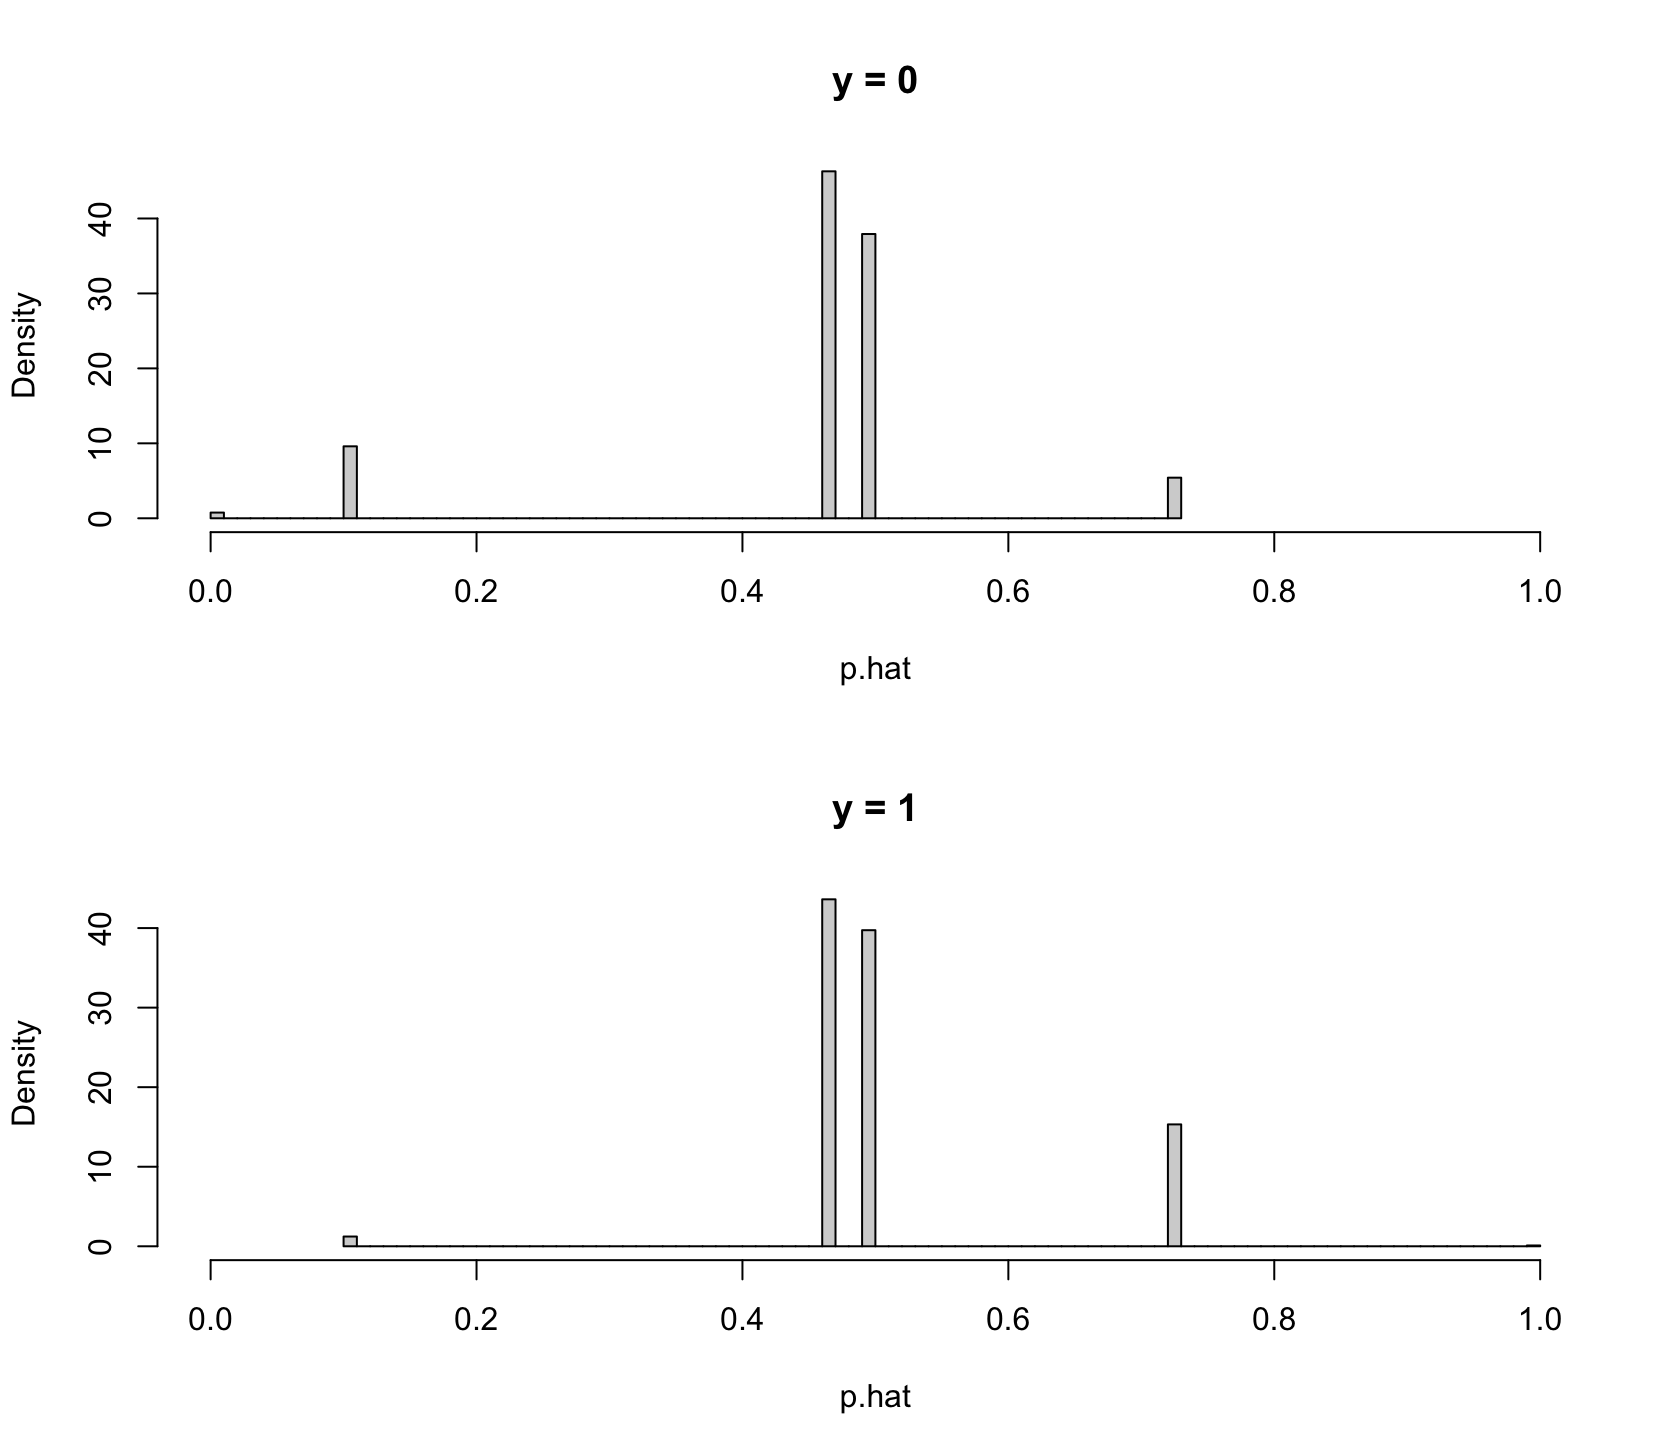
\includegraphics[scale = 0.2]{images/c.png}\]

Plot referenced in part f
\[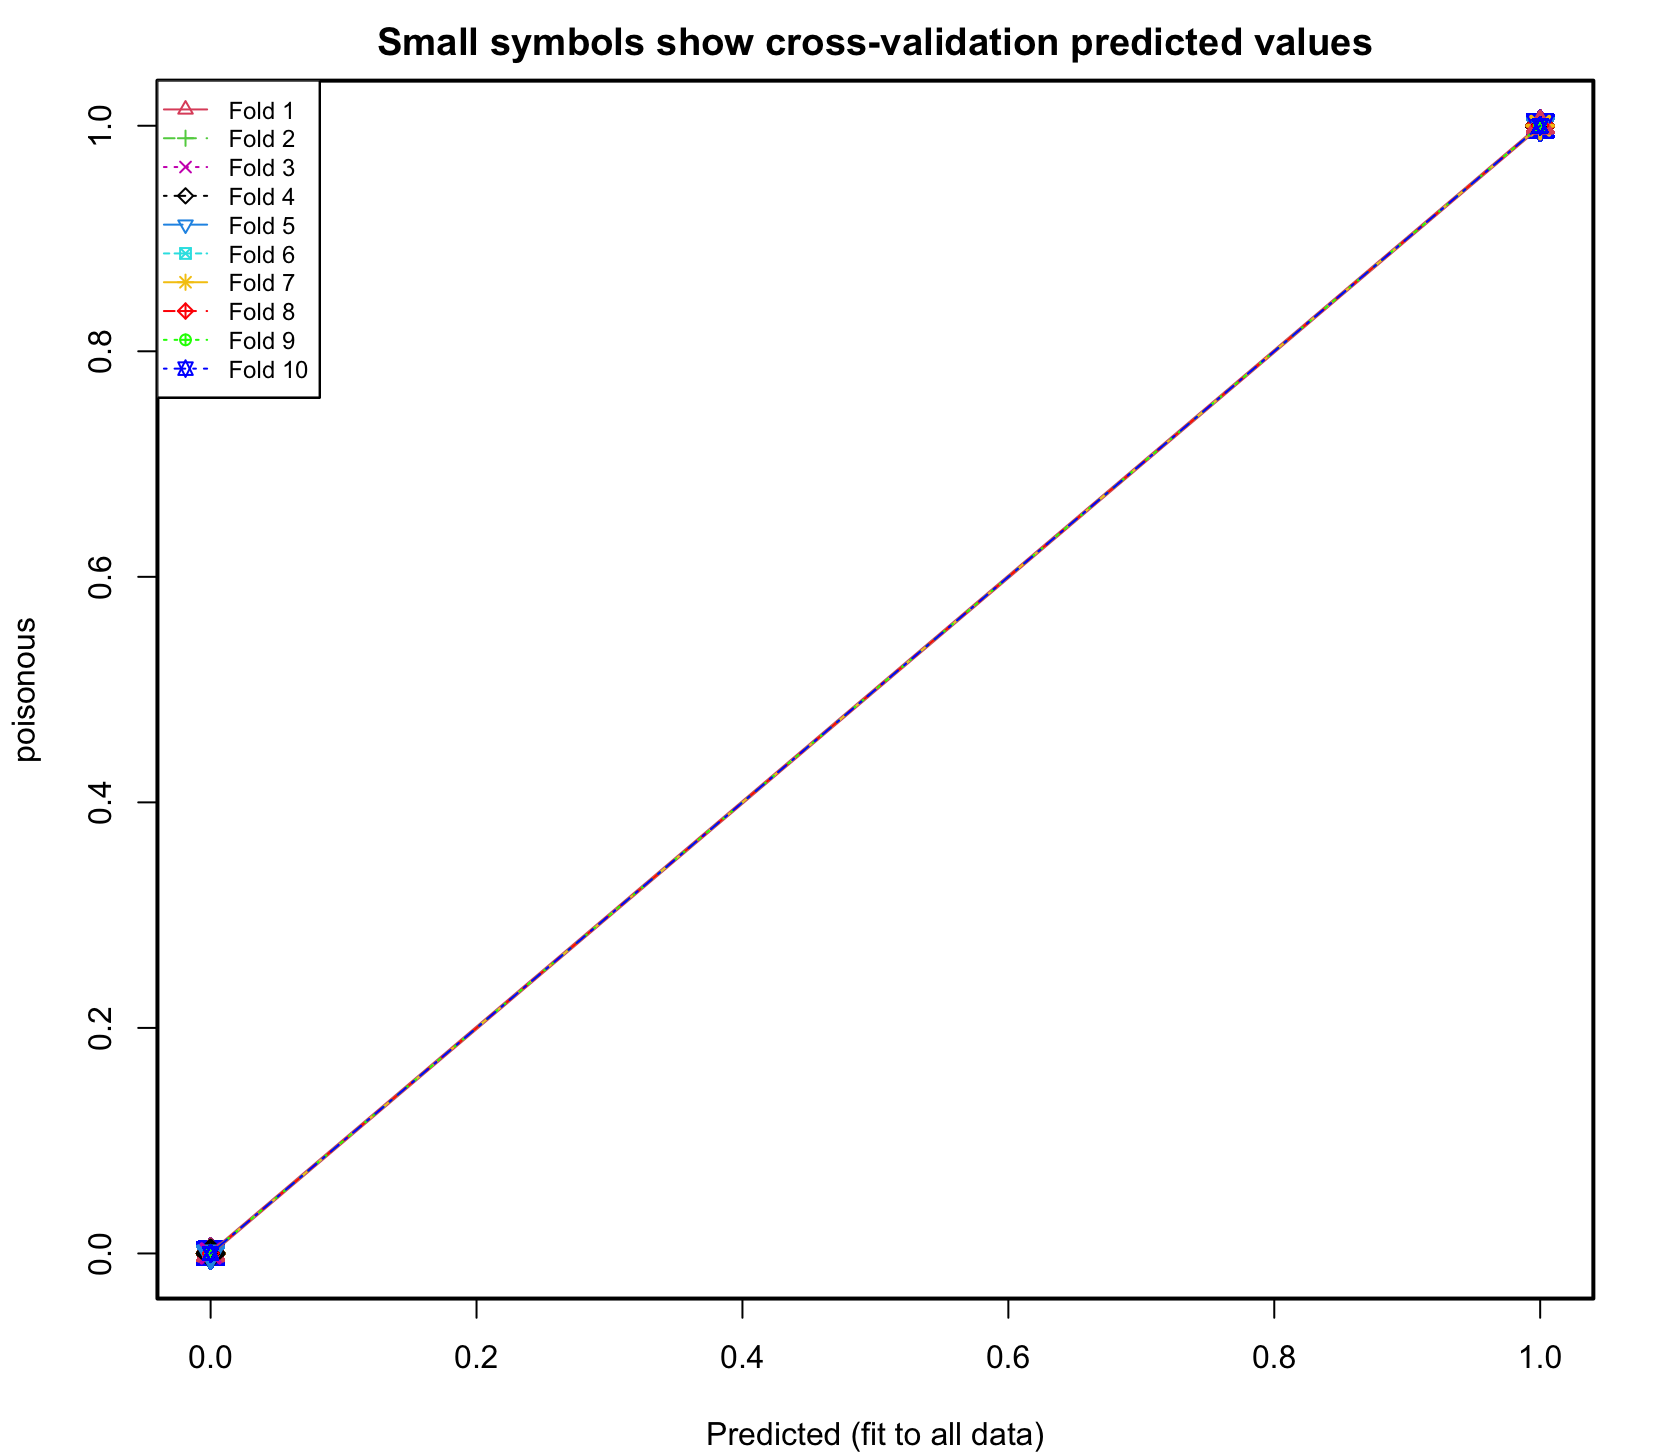
\includegraphics[scale = 0.2]{images/f.png}\]

Code used which was provided by professor Draper. Most comments are deleted to save space, the only modifications were adding comments for when noting some of the FP and FN rates. The code output for the blocks is at the very end after the code. 

\begin{lstlisting}[language = R]
###################### the first block of code starts here #######

# unbuffer the output, if relevant in your R environment

# launch a new copy of R and start with an empty R workspace

rm( list = ls( ) )



raw.mushroom.data <- read.csv( 'stat-206-mushroom-data-2.txt', header = T,
                               stringsAsFactors = T )



str( raw.mushroom.data )



print( 
  
  n <- dim( raw.mushroom.data )[ 1 ] 
  
)



raw.mushroom.data$poisonous <- ifelse( raw.mushroom.data$poisonous == 'p',
                                       1, 0 )


raw.mushroom.data <- subset( raw.mushroom.data, select = - veil.type )

str( raw.mushroom.data )


with( raw.mushroom.data, mean( poisonous ) )


tab.sum <- function( x.1, y ) {
  
  
  stopifnot( length( x.1 ) == length( y ) )
  

  
  summary.function <- function( x ) {
    
    return( list( n = length( x ), mean = mean( x, na.rm = TRUE ), 
                  sd = sd( x, na.rm = TRUE ) ) )
    
  }
  
  map.function <- function( level ) {
    
    indices <- ( x.1 == level )
    
    summary.function( y[ indices ] )
    
  }
  
  levels <- sort( unique( x.1 ) )
  
  out.matrix <- do.call( rbind, Map( map.function, levels ) )
  
  out.matrix <- cbind( levels, out.matrix )
  
  out.matrix <- rbind( out.matrix, c( 'Total', summary.function( y ) ) )
  
  colnames( out.matrix )[ 1 ] <- as.character( substitute( x.1 ) )
  
  return( out.matrix )
  
}



with( raw.mushroom.data, 
      signif( table( cap.shape, useNA = 'always' ) / n, 4 ) )



with( raw.mushroom.data, tab.sum( cap.shape, poisonous ) )

summary( linear.model.1 <- lm( poisonous ~ cap.shape, 
                               data = raw.mushroom.data ) )

p.hat.linear.model.1 <- predict( linear.model.1, type = 'response' )

par( mfrow = c( 2, 1 ) )

hist( p.hat.linear.model.1[ raw.mushroom.data$poisonous == 0 ],
      nclass = 100, main = 'y = 0', xlab = 'p.hat', prob = T,
      xlim = c( 0, 1 ) )

hist( p.hat.linear.model.1[ raw.mushroom.data$poisonous == 1 ],
      nclass = 100, main = 'y = 1', xlab = 'p.hat', prob = T,
      xlim = c( 0, 1 ) )

par( mfrow = c( 1, 1 ) )

pdf( 'stat-206-take-home-test-3-part-2-solutions-figure-1.pdf' )

par( mfrow = c( 2, 1 ) )

hist( p.hat.linear.model.1[ raw.mushroom.data$poisonous == 0 ],
      nclass = 100, main = 'y = 0', xlab = 'p.hat', prob = T,
      xlim = c( 0, 1 ) )

hist( p.hat.linear.model.1[ raw.mushroom.data$poisonous == 1 ],
      nclass = 100, main = 'y = 1', xlab = 'p.hat', prob = T,
      xlim = c( 0, 1 ) )

par( mfrow = c( 1, 1 ) )

dev.off( )


c( mean( p.hat.linear.model.1[ raw.mushroom.data$poisonous == 0 ] ),
   mean( p.hat.linear.model.1[ raw.mushroom.data$poisonous == 1 ] ),
   mean( p.hat.linear.model.1[ raw.mushroom.data$poisonous == 1 ] ) -
     mean( p.hat.linear.model.1[ raw.mushroom.data$poisonous == 0 ] ) )



################ the second block of code ends here #################

################ the third block of code begins here ################

univariate.exploration <- function( new.variable ) {
  
  print( with( raw.mushroom.data, 
               signif( table( new.variable, useNA = 'always' ) / n, 4 ) ) )
  
  print( with( raw.mushroom.data, tab.sum( new.variable, poisonous ) ) )
  
  print( summary( temp.linear.model <- lm( poisonous ~ new.variable, 
                                           data = raw.mushroom.data ) ) )
  
  p.hat.temp.linear.model <- predict( temp.linear.model, type = 'response' )
  
  par( mfrow = c( 2, 1 ) )
  
  hist( p.hat.temp.linear.model[ raw.mushroom.data$poisonous == 0 ],
        nclass = 100, main = 'y = 0', xlab = 'p.hat', prob = T,
        xlim = c( 0, 1 ) )
  
  hist( p.hat.temp.linear.model[ raw.mushroom.data$poisonous == 1 ],
        nclass = 100, main = 'y = 1', xlab = 'p.hat', prob = T,
        xlim = c( 0, 1 ) )
  
  par( mfrow = c( 1, 1 ) )
  
  print( c( 
    mean( p.hat.temp.linear.model[ raw.mushroom.data$poisonous == 0 ] ),
    mean( p.hat.temp.linear.model[ raw.mushroom.data$poisonous == 1 ] ),
    mean( p.hat.temp.linear.model[ raw.mushroom.data$poisonous == 1 ] ) -
    mean( p.hat.temp.linear.model[ raw.mushroom.data$poisonous == 0 ] ) ) )
  
}

with( raw.mushroom.data, univariate.exploration( cap.surface ) )

install.packages( 'R.utils' )

require( R.utils )

predictors <- colnames( raw.mushroom.data )[ 2:22 ]

for ( predictor in predictors) {
  
  printf( "\n\n==============  %s  ==============\n", predictor )
  
  with( raw.mushroom.data, 
        univariate.exploration( eval( parse( text = predictor ) ) ) )
  
}

################ the third block of code ends here #################

############## the fourth block of code begins here ################

summary( linear.model.all.predictors <- lm( poisonous ~ ., 
                                            data = raw.mushroom.data ) )

p.hat.linear.model.all.predictors <- 
  predict( linear.model.all.predictors, type = 'response' )

par( mfrow = c( 2, 1 ) )

hist( p.hat.linear.model.all.predictors[ raw.mushroom.data$poisonous == 0 ],
      nclass = 100, main = 'y = 0', xlab = 'p.hat', prob = T,
      xlim = c( 0, 1 ) )

hist( p.hat.linear.model.all.predictors[ raw.mushroom.data$poisonous == 1 ],
      nclass = 100, main = 'y = 1', xlab = 'p.hat', prob = T,
      xlim = c( 0, 1 ) )

par( mfrow = c( 1, 1 ) )

c( 
  
mean( p.hat.linear.model.all.predictors[ raw.mushroom.data$poisonous == 0 ] ),
mean( p.hat.linear.model.all.predictors[ raw.mushroom.data$poisonous == 1 ] ),
mean( p.hat.linear.model.all.predictors[ raw.mushroom.data$poisonous == 1 ] ) -
mean( p.hat.linear.model.all.predictors[ raw.mushroom.data$poisonous == 0 ] )
  
)

# [1] 2.981711e-13 1.000000e+00 1.000000e+00

############## the fourth block of code ends here #################

############## the fifth block of code begins here ################


dynamic.require <- function( package ) {
  
  if ( eval( parse( text = paste( 'require(', package, ')' ) ) ) ) {
    
    return( 'done' )
    
  }
  
  install.packages( package )
  
  return( eval( parse( text = paste( 'require(', package, ')' ) ) ) )
  
}

dynamic.require( 'DAAG' )

cross.validation.all.predictors.10.fold <- cv.lm( 
  data = raw.mushroom.data, form.lm = formula( poisonous ~ . ), 
  m = 10, printit = F ) 

warnings( )

# Warning messages:
# 1: In predict.lm(subs.lm, newdata = data[rows.out, ]) :
#   prediction from a rank-deficient fit may be misleading
# 2: In predict.lm(subs.lm, newdata = data[rows.out, ]) :
#   prediction from a rank-deficient fit may be misleading
# 3: In predict.lm(subs.lm, newdata = data[rows.out, ]) :
#   prediction from a rank-deficient fit may be misleading
# 4: In predict.lm(subs.lm, newdata = data[rows.out, ]) :
#   prediction from a rank-deficient fit may be misleading
# 5: In predict.lm(subs.lm, newdata = data[rows.out, ]) :
#   prediction from a rank-deficient fit may be misleading
# 6: In predict.lm(subs.lm, newdata = data[rows.out, ]) :
#   prediction from a rank-deficient fit may be misleading
# 7: In predict.lm(subs.lm, newdata = data[rows.out, ]) :
#   prediction from a rank-deficient fit may be misleading
# 8: In predict.lm(subs.lm, newdata = data[rows.out, ]) :
#   prediction from a rank-deficient fit may be misleading
# 9: In predict.lm(subs.lm, newdata = data[rows.out, ]) :
#   prediction from a rank-deficient fit may be misleading
# 10: In predict.lm(subs.lm, newdata = data[rows.out, ]) :
#   prediction from a rank-deficient fit may be misleading
# 11: In cv.lm(data = raw.mushroom.data, form.lm = formula(poisonous ~  ... : 

#  As there is >1 explanatory variable, cross-validation
#  predicted values for a fold are not a linear function
#  of corresponding overall predicted values.  Lines that
#  are shown for the different folds are approximate

# the next function call computes the cross-validated
# root-mean-squared error of the regression predictions,
# which is essentially the same as the value
# from the regression with the full data set

sqrt( attr( cross.validation.all.predictors.10.fold, 'ms' ) )

# [1] 2.199488e-13

############## the fifth block of code ends here ##################

############## the sixth block of code begins here ################

# the next function call investigates which predictors can be dropped
# from the model with little or no predictive accuracy loss

null.model <- lm( poisonous ~ 1, data = raw.mushroom.data )

full.model <- lm( poisonous ~ ., data = raw.mushroom.data )

variable.selection.with.bic <- step( null.model,
                                     scope = list( lower = null.model, 
                                     upper = full.model ), 
                                     direction = 'forward', 
                                     trace = 1, 
                                     steps = 1000, k = log( n ) )

# the output of this function call is in the file

#   stat-206-mushroom-analysis-variable-selection-with-bic.txt

# open this file and study its contents

############## the sixth block of code ends here ##################

############ the seventh block of code begins here ################

summary( linear.model.just.odor <- 
           lm( poisonous ~ odor, data = raw.mushroom.data ) )

# Call:
# lm(formula = poisonous ~ odor, data = raw.mushroom.data)

# Residuals:
#    Min     1Q Median     3Q    Max 
# -0.034 -0.034  0.000  0.000  0.966 

# Coefficients:
#             Estimate Std. Error t value Pr(>|t|)    
# (Intercept) 1.37e-14   5.98e-03    0.00        1    
# odorc       1.00e+00   1.05e-02   95.30  < 2e-16 ***
# odorf       1.00e+00   6.51e-03  153.71  < 2e-16 ***
# odorl       9.37e-14   8.45e-03    0.00        1    
# odorm       1.00e+00   2.08e-02   48.08  < 2e-16 ***
# odorn       3.40e-02   6.31e-03    5.39  7.1e-08 ***
# odorp       1.00e+00   9.57e-03  104.54  < 2e-16 ***
# odors       1.00e+00   7.78e-03  128.55  < 2e-16 ***
# odory       1.00e+00   7.78e-03  128.55  < 2e-16 ***
# ---
# Signif. codes:  0 '***' 0.001 '**' 0.01 '*' 0.05 '.' 0.1 ' ' 1

# Residual standard error: 0.12 on 8115 degrees of freedom
# Multiple R-squared:  0.943,     Adjusted R-squared:  0.943 
# F-statistic: 1.67e+04 on 8 and 8115 DF,  p-value: <2e-16

p.hat.linear.model.just.odor <- 
  predict( linear.model.just.odor, type = 'response' )

par( mfrow = c( 2, 1 ) )

hist( p.hat.linear.model.just.odor[ raw.mushroom.data$poisonous == 0 ],
      nclass = 100, main = 'y = 0', xlab = 'p.hat', prob = T,
      xlim = c( 0, 1 ) )

hist( p.hat.linear.model.just.odor[ raw.mushroom.data$poisonous == 1 ],
      nclass = 100, main = 'y = 1', xlab = 'p.hat', prob = T,
      xlim = c( 0, 1 ) )

par( mfrow = c( 1, 1 ) )

table( p.hat.linear.model.just.odor, useNA = 'always' )

# p.hat.linear.model.just.odor
# 1.36725100485403e-14 1.07412118907621e-13   0.0340136054422548    0.999999999999688 
#                  400                  400                 3528                  192 
#    0.999999999999851     1.00000000000006     1.00000000000009     1.00000000000016 
#                 2160                   36                  576                  576 
#     1.00000000000018                 <NA> 
#                  256                    0 

app.says.poisonous.0.05 <- ifelse( p.hat.linear.model.just.odor > 0.05, 1, 0 )

with( raw.mushroom.data, table( app.says.poisonous.0.05, poisonous ) )

#                        poisonous
# app.says.poisonous.0.05    0    1
#                       0 4208  120
#                       1    0 3796

app.says.poisonous.0.01 <- ifelse( p.hat.linear.model.just.odor > 0.01, 1, 0 )

with( raw.mushroom.data, table( app.says.poisonous.0.01, poisonous ) )
8
#                        poisonous
# app.says.poisonous.0.01    0    1
#                       0  800    0
#                       1 3408 3916

# looking at the best decision rules based on odor and spore print color:

summary( linear.model.odor.spore.print.color <- 
           lm( poisonous ~ odor + spore.print.color, data = raw.mushroom.data ) )

p.hat.linear.model.odor.spore.print.color <- 
  predict( linear.model.odor.spore.print.color, type = 'response' )

par( mfrow = c( 2, 1 ) )

hist( p.hat.linear.model.odor.spore.print.color[ raw.mushroom.data$poisonous == 0 ],
      nclass = 100, main = 'y = 0', xlab = 'p.hat', prob = T,
      xlim = c( 0, 1 ) )

hist( p.hat.linear.model.odor.spore.print.color[ raw.mushroom.data$poisonous == 1 ],
      nclass = 100, main = 'y = 1', xlab = 'p.hat', prob = T,
      xlim = c( 0, 1 ) )

par( mfrow = c( 1, 1 ) )

table( p.hat.linear.model.odor.spore.print.color, useNA = 'always' )

# p.hat.linear.model.odor.spore.print.color
# -2.38704001323558e-14  6.99159606210441e-15  1.71080299696395e-14 
#                    24                   176                   200 
#  6.71763024013884e-14  6.85040678851202e-14  7.00592314937111e-14 
#                    24                    48                    48 
#  7.00838615098795e-14  7.14192263879391e-14  8.15356602954742e-14 
#                    48                  1296                  1344 
#  9.80382985958486e-14  1.08154732503384e-13    0.0646108663730507 
#                   176                   200                    48 
#    0.0719530102790713     0.998042094958255     0.999999999999684 
#                   624                  1584                    96 
#     0.999999999999694      1.00000000000006      1.00000000000007 
#                    96                    36                    72 
#      1.00000000000009      1.00000000000016      1.00000000000018 
#                   576                   576                   128 
#      1.00000000000019      1.00538423886428                  <NA> 
#                   128                   576                     0

odor.spore.print.color.app.says.poisonous.0.05 <- 
  ifelse( p.hat.linear.model.odor.spore.print.color > 0.05, 1, 0 )

with( raw.mushroom.data, table( odor.spore.print.color.app.says.poisonous.0.05, 
                                poisonous ) )

#                                               poisonous
# odor.spore.print.color.app.says.poisonous.0.05    0    1
#                                              0 3584    0
#                                              1  624 3916

odor.spore.print.color.app.says.poisonous.0.07 <- 
  ifelse( p.hat.linear.model.odor.spore.print.color > 0.07, 1, 0 )

with( raw.mushroom.data, table( odor.spore.print.color.app.says.poisonous.0.07, 
                                poisonous ) )

#                                               poisonous
# odor.spore.print.color.app.says.poisonous.0.07    0    1
#                                              0 3632    0
#                                              1  576 3916

# 0.05 Cutoff 
#      1    0 
# 1 - 3916 624 
# 0 -  0   3584
# FP = 0.1483
# FN = 0 
#
# 0.07 Cutoff
#       1     0
# 1 - 3916   576
# 0 -  0    3631
# FP = 0.1369
# FN = 0 
#

odor.spore.print.color.app.says.poisonous.0.08 <- 
  ifelse( p.hat.linear.model.odor.spore.print.color > 0.08, 1, 0 )

with( raw.mushroom.data, table( odor.spore.print.color.app.says.poisonous.0.08, 
                                poisonous ) )

#                                               poisonous
# odor.spore.print.color.app.says.poisonous.0.08    0    1
#                                              0 4208   48
#                                              1    0 3868
# 0.08 Cutoff
#       1      0
# 1 - 3868     0
# 0 -  48     4208
#
# FP = 0
# FN = 0.0123
############## the seventh block of code ends here ################


\end{lstlisting}

\textbf{CODE OUTPUT======================}

\begin{lstlisting}[language = R]
    'data.frame':	8124 obs. of  23 variables:
 $ poisonous               : Factor w/ 2 levels "e","p": 2 1 1 2 1 1 1 1 2 1 ...
 $ cap.shape               : Factor w/ 6 levels "b","c","f","k",..: 6 6 1 6 6 6 1 1 6 1 ...
 $ cap.surface             : Factor w/ 4 levels "f","g","s","y": 3 3 3 4 3 4 3 4 4 3 ...
 $ cap.color               : Factor w/ 10 levels "b","c","e","g",..: 5 10 9 9 4 10 9 9 9 10 ...
 $ bruises                 : Factor w/ 2 levels "f","t": 2 2 2 2 1 2 2 2 2 2 ...
 $ odor                    : Factor w/ 9 levels "a","c","f","l",..: 7 1 4 7 6 1 1 4 7 1 ...
 $ gill.attachment         : Factor w/ 2 levels "a","f": 2 2 2 2 2 2 2 2 2 2 ...
 $ gill.spacing            : Factor w/ 2 levels "c","w": 1 1 1 1 2 1 1 1 1 1 ...
 $ gill.size               : Factor w/ 2 levels "b","n": 2 1 1 2 1 1 1 1 2 1 ...
 $ gill.color              : Factor w/ 12 levels "b","e","g","h",..: 5 5 6 6 5 6 3 6 8 3 ...
 $ stalk.shape             : Factor w/ 2 levels "e","t": 1 1 1 1 2 1 1 1 1 1 ...
 $ stalk.root              : Factor w/ 5 levels "?","b","c","e",..: 4 3 3 4 4 3 3 3 4 3 ...
 $ stalk.surface.above.ring: Factor w/ 4 levels "f","k","s","y": 3 3 3 3 3 3 3 3 3 3 ...
 $ stalk.surface.below.ring: Factor w/ 4 levels "f","k","s","y": 3 3 3 3 3 3 3 3 3 3 ...
 $ stalk.color.above.ring  : Factor w/ 9 levels "b","c","e","g",..: 8 8 8 8 8 8 8 8 8 8 ...
 $ stalk.color.below.ring  : Factor w/ 9 levels "b","c","e","g",..: 8 8 8 8 8 8 8 8 8 8 ...
 $ veil.type               : Factor w/ 1 level "p": 1 1 1 1 1 1 1 1 1 1 ...
 $ veil.color              : Factor w/ 4 levels "n","o","w","y": 3 3 3 3 3 3 3 3 3 3 ...
 $ ring.number             : Factor w/ 3 levels "n","o","t": 2 2 2 2 2 2 2 2 2 2 ...
 $ ring.type               : Factor w/ 5 levels "e","f","l","n",..: 5 5 5 5 1 5 5 5 5 5 ...
 $ spore.print.color       : Factor w/ 9 levels "b","h","k","n",..: 3 4 4 3 4 3 3 4 3 3 ...
 $ population              : Factor w/ 6 levels "a","c","n","s",..: 4 3 3 4 1 3 3 4 5 4 ...
 $ habitat                 : Factor w/ 7 levels "d","g","l","m",..: 6 2 4 6 2 2 4 4 2 4 ...
[1] 8124
'data.frame':	8124 obs. of  22 variables:
 $ poisonous               : num  1 0 0 1 0 0 0 0 1 0 ...
 $ cap.shape               : Factor w/ 6 levels "b","c","f","k",..: 6 6 1 6 6 6 1 1 6 1 ...
 $ cap.surface             : Factor w/ 4 levels "f","g","s","y": 3 3 3 4 3 4 3 4 4 3 ...
 $ cap.color               : Factor w/ 10 levels "b","c","e","g",..: 5 10 9 9 4 10 9 9 9 10 ...
 $ bruises                 : Factor w/ 2 levels "f","t": 2 2 2 2 1 2 2 2 2 2 ...
 $ odor                    : Factor w/ 9 levels "a","c","f","l",..: 7 1 4 7 6 1 1 4 7 1 ...
 $ gill.attachment         : Factor w/ 2 levels "a","f": 2 2 2 2 2 2 2 2 2 2 ...
 $ gill.spacing            : Factor w/ 2 levels "c","w": 1 1 1 1 2 1 1 1 1 1 ...
 $ gill.size               : Factor w/ 2 levels "b","n": 2 1 1 2 1 1 1 1 2 1 ...
 $ gill.color              : Factor w/ 12 levels "b","e","g","h",..: 5 5 6 6 5 6 3 6 8 3 ...
 $ stalk.shape             : Factor w/ 2 levels "e","t": 1 1 1 1 2 1 1 1 1 1 ...
 $ stalk.root              : Factor w/ 5 levels "?","b","c","e",..: 4 3 3 4 4 3 3 3 4 3 ...
 $ stalk.surface.above.ring: Factor w/ 4 levels "f","k","s","y": 3 3 3 3 3 3 3 3 3 3 ...
 $ stalk.surface.below.ring: Factor w/ 4 levels "f","k","s","y": 3 3 3 3 3 3 3 3 3 3 ...
 $ stalk.color.above.ring  : Factor w/ 9 levels "b","c","e","g",..: 8 8 8 8 8 8 8 8 8 8 ...
 $ stalk.color.below.ring  : Factor w/ 9 levels "b","c","e","g",..: 8 8 8 8 8 8 8 8 8 8 ...
 $ veil.color              : Factor w/ 4 levels "n","o","w","y": 3 3 3 3 3 3 3 3 3 3 ...
 $ ring.number             : Factor w/ 3 levels "n","o","t": 2 2 2 2 2 2 2 2 2 2 ...
 $ ring.type               : Factor w/ 5 levels "e","f","l","n",..: 5 5 5 5 1 5 5 5 5 5 ...
 $ spore.print.color       : Factor w/ 9 levels "b","h","k","n",..: 3 4 4 3 4 3 3 4 3 3 ...
 $ population              : Factor w/ 6 levels "a","c","n","s",..: 4 3 3 4 1 3 3 4 5 4 ...
 $ habitat                 : Factor w/ 7 levels "d","g","l","m",..: 6 2 4 6 2 2 4 4 2 4 ...
new.variable
        f         g         s         y      <NA> 
0.2856000 0.0004924 0.3146000 0.3993000 0.0000000 
     new.variable n    mean      sd       
[1,] 1            2320 0.3275862 0.4694342
[2,] 2            4    1         0        
[3,] 3            2556 0.5524257 0.4973413
[4,] 4            3244 0.5363748 0.498752 
[5,] "Total"      8124 0.4820286 0.4997077

Call:
lm(formula = poisonous ~ new.variable, data = raw.mushroom.data)

Residuals:
    Min      1Q  Median      3Q     Max 
-0.5524 -0.5364 -0.3276  0.4636  0.6724 

Coefficients:
              Estimate Std. Error t value Pr(>|t|)    
(Intercept)    0.32759    0.01017  32.200  < 2e-16 ***
new.variableg  0.67241    0.24522   2.742  0.00612 ** 
new.variables  0.22484    0.01405  16.001  < 2e-16 ***
new.variabley  0.20879    0.01332  15.671  < 2e-16 ***
---


Residual standard error: 0.49 on 8120 degrees of freedom
Multiple R-squared:  0.03878,	Adjusted R-squared:  0.03842 
F-statistic: 109.2 on 3 and 8120 DF,  p-value: < 2.2e-16

[1] 0.46333584 0.50211511 0.03877928
Error in install.packages : Updating loaded packages


==============  cap.shape  ==============
new.variable
        b         c         f         k         s         x      <NA> 
0.0556400 0.0004924 0.3880000 0.1019000 0.0039390 0.4500000 0.0000000 
     new.variable n    mean      sd       
[1,] 1            452  0.1061947 0.308428 
[2,] 2            4    1         0        
[3,] 3            3152 0.4936548 0.5000391
[4,] 4            828  0.7246377 0.4469667
[5,] 5            32   0         0        
[6,] 6            3656 0.4671772 0.4989898
[7,] "Total"      8124 0.4820286 0.4997077

Call:
lm(formula = poisonous ~ new.variable, data = raw.mushroom.data)

Residuals:
    Min      1Q  Median      3Q     Max 
-0.7246 -0.4672 -0.1062  0.5063  0.8938 

Coefficients:
              Estimate Std. Error t value Pr(>|t|)    
(Intercept)    0.10619    0.02279   4.659 3.22e-06 ***
new.variablec  0.89381    0.24335   3.673 0.000241 ***
new.variablef  0.38746    0.02437  15.898  < 2e-16 ***
new.variablek  0.61844    0.02834  21.824  < 2e-16 ***
new.variables -0.10619    0.08864  -1.198 0.230926    
new.variablex  0.36098    0.02416  14.942  < 2e-16 ***
---


Residual standard error: 0.4846 on 8118 degrees of freedom
Multiple R-squared:  0.06031,	Adjusted R-squared:  0.05973 
F-statistic: 104.2 on 5 and 8118 DF,  p-value: < 2.2e-16

[1] 0.45295970 0.51326496 0.06030526


==============  cap.surface  ==============
new.variable
        f         g         s         y      <NA> 
0.2856000 0.0004924 0.3146000 0.3993000 0.0000000 
     new.variable n    mean      sd       
[1,] 1            2320 0.3275862 0.4694342
[2,] 2            4    1         0        
[3,] 3            2556 0.5524257 0.4973413
[4,] 4            3244 0.5363748 0.498752 
[5,] "Total"      8124 0.4820286 0.4997077

Call:
lm(formula = poisonous ~ new.variable, data = raw.mushroom.data)

Residuals:
    Min      1Q  Median      3Q     Max 
-0.5524 -0.5364 -0.3276  0.4636  0.6724 

Coefficients:
              Estimate Std. Error t value Pr(>|t|)    
(Intercept)    0.32759    0.01017  32.200  < 2e-16 ***
new.variableg  0.67241    0.24522   2.742  0.00612 ** 
new.variables  0.22484    0.01405  16.001  < 2e-16 ***
new.variabley  0.20879    0.01332  15.671  < 2e-16 ***
---


Residual standard error: 0.49 on 8120 degrees of freedom
Multiple R-squared:  0.03878,	Adjusted R-squared:  0.03842 
F-statistic: 109.2 on 3 and 8120 DF,  p-value: < 2.2e-16

[1] 0.46333584 0.50211511 0.03877928


==============  cap.color  ==============
new.variable
       b        c        e        g        n        p        r        u        w        y     <NA> 
0.020680 0.005416 0.184600 0.226500 0.281100 0.017730 0.001969 0.001969 0.128000 0.132000 0.000000 
      new.variable n    mean      sd       
 [1,] 1            168  0.7142857 0.4531045
 [2,] 2            44   0.2727273 0.4505106
 [3,] 3            1500 0.584     0.4930579
 [4,] 4            1840 0.4391304 0.496416 
 [5,] 5            2284 0.4465849 0.4972475
 [6,] 6            144  0.6111111 0.4891996
 [7,] 7            16   0         0        
 [8,] 8            16   0         0        
 [9,] 9            1040 0.3076923 0.4617605
[10,] 10           1072 0.6268657 0.4838631
[11,] "Total"      8124 0.4820286 0.4997077

Call:
lm(formula = poisonous ~ new.variable, data = raw.mushroom.data)

Residuals:
    Min      1Q  Median      3Q     Max 
-0.7143 -0.4466 -0.3077  0.5534  0.7273 

Coefficients:
              Estimate Std. Error t value Pr(>|t|)    
(Intercept)    0.71429    0.03764  18.975  < 2e-16 ***
new.variablec -0.44156    0.08263  -5.344 9.34e-08 ***
new.variablee -0.13029    0.03970  -3.282  0.00103 ** 
new.variableg -0.27516    0.03932  -6.997 2.82e-12 ***
new.variablen -0.26770    0.03900  -6.864 7.21e-12 ***
new.variablep -0.10317    0.05541  -1.862  0.06263 .  
new.variabler -0.71429    0.12765  -5.595 2.27e-08 ***
new.variableu -0.71429    0.12765  -5.595 2.27e-08 ***
new.variablew -0.40659    0.04057 -10.022  < 2e-16 ***
new.variabley -0.08742    0.04049  -2.159  0.03086 *  
---


Residual standard error: 0.4879 on 8114 degrees of freedom
Multiple R-squared:  0.04771,	Adjusted R-squared:  0.04665 
F-statistic: 45.17 on 9 and 8114 DF,  p-value: < 2.2e-16

[1] 0.45903087 0.50674109 0.04771021


==============  bruises  ==============
new.variable
     f      t   <NA> 
0.5844 0.4156 0.0000 
     new.variable n    mean      sd       
[1,] 1            4748 0.6933446 0.4611536
[2,] 2            3376 0.1848341 0.3882204
[3,] "Total"      8124 0.4820286 0.4997077

Call:
lm(formula = poisonous ~ new.variable, data = raw.mushroom.data)

Residuals:
    Min      1Q  Median      3Q     Max 
-0.6933 -0.1848 -0.1848  0.3067  0.8152 

Coefficients:
               Estimate Std. Error t value Pr(>|t|)    
(Intercept)    0.693345   0.006274  110.50   <2e-16 ***
new.variablet -0.508510   0.009733  -52.24   <2e-16 ***
---


Residual standard error: 0.4323 on 8122 degrees of freedom
Multiple R-squared:  0.2515,	Adjusted R-squared:  0.2514 
F-statistic:  2730 on 1 and 8122 DF,  p-value: < 2.2e-16

[1] 0.3607826 0.6123153 0.2515327


==============  odor  ==============
new.variable
       a        c        f        l        m        n        p        s        y     <NA> 
0.049240 0.023630 0.265900 0.049240 0.004431 0.434300 0.031510 0.070900 0.070900 0.000000 
      new.variable n    mean       sd       
 [1,] 1            400  0          0        
 [2,] 2            192  1          0        
 [3,] 3            2160 1          0        
 [4,] 4            400  0          0        
 [5,] 5            36   1          0        
 [6,] 6            3528 0.03401361 0.1812898
 [7,] 7            256  1          0        
 [8,] 8            576  1          0        
 [9,] 9            576  1          0        
[10,] "Total"      8124 0.4820286  0.4997077

Call:
lm(formula = poisonous ~ new.variable, data = raw.mushroom.data)

Residuals:
     Min       1Q   Median       3Q      Max 
-0.03401 -0.03401  0.00000  0.00000  0.96599 

Coefficients:
               Estimate Std. Error t value Pr(>|t|)    
(Intercept)   1.366e-14  5.976e-03   0.000        1    
new.variablec 1.000e+00  1.049e-02  95.299  < 2e-16 ***
new.variablef 1.000e+00  6.506e-03 153.711  < 2e-16 ***
new.variablel 9.370e-14  8.451e-03   0.000        1    
new.variablem 1.000e+00  2.080e-02  48.085  < 2e-16 ***
new.variablen 3.401e-02  6.306e-03   5.394 7.08e-08 ***
new.variablep 1.000e+00  9.566e-03 104.536  < 2e-16 ***
new.variables 1.000e+00  7.779e-03 128.554  < 2e-16 ***
new.variabley 1.000e+00  7.779e-03 128.554  < 2e-16 ***
---


Residual standard error: 0.1195 on 8115 degrees of freedom
Multiple R-squared:  0.9429,	Adjusted R-squared:  0.9428 
F-statistic: 1.674e+04 on 8 and 8115 DF,  p-value: < 2.2e-16

[1] 0.02754714 0.97039878 0.94285164


==============  gill.attachment  ==============
new.variable
      a       f    <NA> 
0.02585 0.97420 0.00000 
     new.variable n    mean       sd       
[1,] 1            210  0.08571429 0.2806106
[2,] 2            7914 0.4925449  0.499976 
[3,] "Total"      8124 0.4820286  0.4997077

Call:
lm(formula = poisonous ~ new.variable, data = raw.mushroom.data)

Residuals:
     Min       1Q   Median       3Q      Max 
-0.49254 -0.49254 -0.08571  0.50746  0.91429 

Coefficients:
              Estimate Std. Error t value Pr(>|t|)    
(Intercept)    0.08571    0.03420   2.507   0.0122 *  
new.variablef  0.40683    0.03465  11.742   <2e-16 ***
---


Residual standard error: 0.4955 on 8122 degrees of freedom
Multiple R-squared:  0.01669,	Adjusted R-squared:  0.01657 
F-statistic: 137.9 on 1 and 8122 DF,  p-value: < 2.2e-16

[1] 0.4739822 0.4906748 0.0166926


==============  gill.spacing  ==============
new.variable
     c      w   <NA> 
0.8385 0.1615 0.0000 
     new.variable n    mean       sd       
[1,] 1            6812 0.5584263  0.4966111
[2,] 2            1312 0.08536585 0.2795319
[3,] "Total"      8124 0.4820286  0.4997077

Call:
lm(formula = poisonous ~ new.variable, data = raw.mushroom.data)

Residuals:
     Min       1Q   Median       3Q      Max 
-0.55843 -0.55843 -0.08537  0.44157  0.91463 

Coefficients:
               Estimate Std. Error t value Pr(>|t|)    
(Intercept)    0.558426   0.005676   98.39   <2e-16 ***
new.variablew -0.473060   0.014123  -33.50   <2e-16 ***
---


Residual standard error: 0.4684 on 8122 degrees of freedom
Multiple R-squared:  0.1214,	Adjusted R-squared:  0.1213 
F-statistic:  1122 on 1 and 8122 DF,  p-value: < 2.2e-16

[1] 0.4235231 0.5448965 0.1213734


==============  gill.size  ==============
new.variable
     b      n   <NA> 
0.6908 0.3092 0.0000 
     new.variable n    mean      sd       
[1,] 1            5612 0.3014968 0.4589488
[2,] 2            2512 0.8853503 0.3186621
[3,] "Total"      8124 0.4820286 0.4997077

Call:
lm(formula = poisonous ~ new.variable, data = raw.mushroom.data)

Residuals:
    Min      1Q  Median      3Q     Max 
-0.8853 -0.3015 -0.3015  0.1147  0.6985 

Coefficients:
              Estimate Std. Error t value Pr(>|t|)    
(Intercept)   0.301497   0.005615   53.70   <2e-16 ***
new.variablen 0.583854   0.010097   57.83   <2e-16 ***
---


Residual standard error: 0.4206 on 8122 degrees of freedom
Multiple R-squared:  0.2916,	Adjusted R-squared:  0.2915 
F-statistic:  3344 on 1 and 8122 DF,  p-value: < 2.2e-16

[1] 0.3414563 0.6330827 0.2916263


==============  gill.color  ==============
new.variable
       b        e        g        h        k        n        o        p        r        u        w        y     <NA> 
0.212700 0.011820 0.092570 0.090100 0.050220 0.129000 0.007878 0.183700 0.002954 0.060560 0.148000 0.010590 0.000000 
      new.variable n    mean       sd       
 [1,] 1            1728 1          0        
 [2,] 2            96   0          0        
 [3,] 3            752  0.6702128  0.4704486
 [4,] 4            732  0.7213115  0.4486605
 [5,] 5            408  0.1568627  0.3641178
 [6,] 6            1048 0.1068702  0.3090957
 [7,] 7            64   0          0        
 [8,] 8            1492 0.4289544  0.4950927
 [9,] 9            24   1          0        
[10,] 10           492  0.09756098 0.2970221
[11,] 11           1202 0.2046589  0.4036201
[12,] 12           86   0.255814   0.4388768
[13,] "Total"      8124 0.4820286  0.4997077

Call:
lm(formula = poisonous ~ new.variable, data = raw.mushroom.data)

Residuals:
    Min      1Q  Median      3Q     Max 
-0.7213 -0.2047  0.0000  0.2787  0.9024 

Coefficients:
                Estimate Std. Error t value Pr(>|t|)    
(Intercept)    1.000e+00  8.811e-03  113.50   <2e-16 ***
new.variablee -1.000e+00  3.841e-02  -26.04   <2e-16 ***
new.variableg -3.298e-01  1.600e-02  -20.61   <2e-16 ***
new.variableh -2.787e-01  1.615e-02  -17.25   <2e-16 ***
new.variablek -8.431e-01  2.016e-02  -41.82   <2e-16 ***
new.variablen -8.931e-01  1.434e-02  -62.28   <2e-16 ***
new.variableo -1.000e+00  4.662e-02  -21.45   <2e-16 ***
new.variablep -5.710e-01  1.294e-02  -44.12   <2e-16 ***
new.variabler  1.469e-14  7.528e-02    0.00        1    
new.variableu -9.024e-01  1.872e-02  -48.22   <2e-16 ***
new.variablew -7.953e-01  1.376e-02  -57.82   <2e-16 ***
new.variabley -7.442e-01  4.047e-02  -18.39   <2e-16 ***
---


Residual standard error: 0.3663 on 8112 degrees of freedom
Multiple R-squared:  0.4635,	Adjusted R-squared:  0.4628 
F-statistic: 637.2 on 11 and 8112 DF,  p-value: < 2.2e-16

[1] 0.2585941 0.7221236 0.4635296


==============  stalk.shape  ==============
new.variable
     e      t   <NA> 
0.4328 0.5672 0.0000 
     new.variable n    mean      sd       
[1,] 1            3516 0.5403868 0.4984371
[2,] 2            4608 0.4375    0.4961322
[3,] "Total"      8124 0.4820286 0.4997077

Call:
lm(formula = poisonous ~ new.variable, data = raw.mushroom.data)

Residuals:
    Min      1Q  Median      3Q     Max 
-0.5404 -0.4375 -0.4375  0.4596  0.5625 

Coefficients:
               Estimate Std. Error t value Pr(>|t|)    
(Intercept)    0.540387   0.008384  64.455   <2e-16 ***
new.variablet -0.102887   0.011132  -9.242   <2e-16 ***
---


Residual standard error: 0.4971 on 8122 degrees of freedom
Multiple R-squared:  0.01041,	Adjusted R-squared:  0.01029 
F-statistic: 85.42 on 1 and 8122 DF,  p-value: < 2.2e-16

[1] 0.47701166 0.48741954 0.01040788


==============  stalk.root  ==============
new.variable
      ?       b       c       e       r    <NA> 
0.30530 0.46480 0.06844 0.13790 0.02363 0.00000 
     new.variable n    mean       sd       
[1,] 1            2480 0.7096774  0.4540027
[2,] 2            3776 0.4915254  0.4999944
[3,] 3            556  0.07913669 0.2701951
[4,] 4            1120 0.2285714  0.4201001
[5,] 5            192  0          0        
[6,] "Total"      8124 0.4820286  0.4997077

Call:
lm(formula = poisonous ~ new.variable, data = raw.mushroom.data)

Residuals:
    Min      1Q  Median      3Q     Max 
-0.7097 -0.4915  0.0000  0.5085  0.9209 

Coefficients:
               Estimate Std. Error t value Pr(>|t|)    
(Intercept)    0.709677   0.009169   77.40   <2e-16 ***
new.variableb -0.218152   0.011802  -18.48   <2e-16 ***
new.variablec -0.630541   0.021425  -29.43   <2e-16 ***
new.variablee -0.481106   0.016438  -29.27   <2e-16 ***
new.variabler -0.709677   0.034204  -20.75   <2e-16 ***
---


Residual standard error: 0.4566 on 8119 degrees of freedom
Multiple R-squared:  0.1655,	Adjusted R-squared:  0.1651 
F-statistic: 402.5 on 4 and 8119 DF,  p-value: < 2.2e-16

[1] 0.4022577 0.5677476 0.1654900


==============  stalk.surface.above.ring  ==============
new.variable
       f        k        s        y     <NA> 
0.067950 0.292000 0.637100 0.002954 0.000000 
     new.variable n    mean      sd       
[1,] 1            552  0.2608696 0.4395072
[2,] 2            2372 0.9392917 0.2388448
[3,] 3            5176 0.2967543 0.4568714
[4,] 4            24   0.3333333 0.4815434
[5,] "Total"      8124 0.4820286 0.4997077

Call:
lm(formula = poisonous ~ new.variable, data = raw.mushroom.data)

Residuals:
     Min       1Q   Median       3Q      Max 
-0.93929 -0.29675 -0.26087  0.06071  0.73913 

Coefficients:
              Estimate Std. Error t value Pr(>|t|)    
(Intercept)    0.26087    0.01721  15.160   <2e-16 ***
new.variablek  0.67842    0.01911  35.510   <2e-16 ***
new.variables  0.03588    0.01810   1.982   0.0475 *  
new.variabley  0.07246    0.08430   0.860   0.3900    
---


Residual standard error: 0.4043 on 8120 degrees of freedom
Multiple R-squared:  0.3457,	Adjusted R-squared:  0.3454 
F-statistic:  1430 on 3 and 8120 DF,  p-value: < 2.2e-16

[1] 0.3154020 0.6610798 0.3456778


==============  stalk.surface.below.ring  ==============
new.variable
      f       k       s       y    <NA> 
0.07386 0.28360 0.60760 0.03496 0.00000 
     new.variable n    mean      sd       
[1,] 1            600  0.24      0.4274395
[2,] 2            2304 0.9375    0.242114 
[3,] 3            4936 0.3111831 0.4630244
[4,] 4            284  0.2676056 0.4434923
[5,] "Total"      8124 0.4820286 0.4997077

Call:
lm(formula = poisonous ~ new.variable, data = raw.mushroom.data)

Residuals:
    Min      1Q  Median      3Q     Max 
-0.9375 -0.3112 -0.2400  0.0625  0.7600 

Coefficients:
              Estimate Std. Error t value Pr(>|t|)    
(Intercept)    0.24000    0.01670  14.375  < 2e-16 ***
new.variablek  0.69750    0.01874  37.211  < 2e-16 ***
new.variables  0.07118    0.01768   4.026 5.73e-05 ***
new.variabley  0.02761    0.02946   0.937    0.349    
---

Residual standard error: 0.409 on 8120 degrees of freedom
Multiple R-squared:  0.3304,	Adjusted R-squared:  0.3302 
F-statistic:  1336 on 3 and 8120 DF,  p-value: < 2.2e-16

[1] 0.3227483 0.6531857 0.3304375


==============  stalk.color.above.ring  ==============
new.variable
        b         c         e         g         n         o         p         w         y      <NA> 
0.0531800 0.0044310 0.0118200 0.0709000 0.0551500 0.0236300 0.2304000 0.5495000 0.0009847 0.0000000 
      new.variable n    mean      sd       
 [1,] 1            432  1         0        
 [2,] 2            36   1         0        
 [3,] 3            96   0         0        
 [4,] 4            576  0         0        
 [5,] 5            448  0.9642857 0.1857843
 [6,] 6            192  0         0        
 [7,] 7            1872 0.6923077 0.4616618
 [8,] 8            4464 0.3835125 0.4862958
 [9,] 9            8    1         0        
[10,] "Total"      8124 0.4820286 0.4997077

Call:
lm(formula = poisonous ~ new.variable, data = raw.mushroom.data)

Residuals:
    Min      1Q  Median      3Q     Max 
-0.9643 -0.3835  0.0000  0.3077  0.6165 

Coefficients:
                Estimate Std. Error t value Pr(>|t|)    
(Intercept)    1.000e+00  2.047e-02  48.841   <2e-16 ***
new.variablec  9.813e-14  7.382e-02   0.000    1.000    
new.variablee -1.000e+00  4.802e-02 -20.826   <2e-16 ***
new.variableg -1.000e+00  2.709e-02 -36.920   <2e-16 ***
new.variablen -3.571e-02  2.870e-02  -1.245    0.213    
new.variableo -1.000e+00  3.691e-02 -27.092   <2e-16 ***
new.variablep -3.077e-01  2.271e-02 -13.546   <2e-16 ***
new.variablew -6.165e-01  2.144e-02 -28.751   <2e-16 ***
new.variabley -2.260e-14  1.518e-01   0.000    1.000    
---


Residual standard error: 0.4256 on 8115 degrees of freedom
Multiple R-squared:  0.2755,	Adjusted R-squared:  0.2748 
F-statistic: 385.7 on 8 and 8115 DF,  p-value: < 2.2e-16

[1] 0.3492453 0.6247129 0.2754676


==============  stalk.color.below.ring  ==============
new.variable
       b        c        e        g        n        o        p        w        y     <NA> 
0.053180 0.004431 0.011820 0.070900 0.063020 0.023630 0.230400 0.539600 0.002954 0.000000 
      new.variable n    mean      sd       
 [1,] 1            432  1         0        
 [2,] 2            36   1         0        
 [3,] 3            96   0         0        
 [4,] 4            576  0         0        
 [5,] 5            512  0.875     0.3310424
 [6,] 6            192  0         0        
 [7,] 7            1872 0.6923077 0.4616618
 [8,] 8            4384 0.3832117 0.4862247
 [9,] 9            24   1         0        
[10,] "Total"      8124 0.4820286 0.4997077

Call:
lm(formula = poisonous ~ new.variable, data = raw.mushroom.data)

Residuals:
    Min      1Q  Median      3Q     Max 
-0.8750 -0.3832  0.0000  0.3077  0.6168 

Coefficients:
                Estimate Std. Error t value Pr(>|t|)    
(Intercept)    1.000e+00  2.062e-02  48.490  < 2e-16 ***
new.variablec  4.091e-14  7.436e-02   0.000        1    
new.variablee -1.000e+00  4.836e-02 -20.676  < 2e-16 ***
new.variableg -1.000e+00  2.728e-02 -36.655  < 2e-16 ***
new.variablen -1.250e-01  2.800e-02  -4.464 8.16e-06 ***
new.variableo -1.000e+00  3.718e-02 -26.897  < 2e-16 ***
new.variablep -3.077e-01  2.288e-02 -13.449  < 2e-16 ***
new.variablew -6.168e-01  2.162e-02 -28.535  < 2e-16 ***
new.variabley -1.192e-14  8.989e-02   0.000        1    
---

Residual standard error: 0.4286 on 8115 degrees of freedom
Multiple R-squared:  0.2649,	Adjusted R-squared:  0.2642 
F-statistic: 365.6 on 8 and 8115 DF,  p-value: < 2.2e-16

[1] 0.3543188 0.6192611 0.2649423


==============  veil.color  ==============
new.variable
        n         o         w         y      <NA> 
0.0118200 0.0118200 0.9754000 0.0009847 0.0000000 
     new.variable n    mean      sd       
[1,] 1            96   0         0        
[2,] 2            96   0         0        
[3,] 3            7924 0.4931853 0.4999851
[4,] 4            8    1         0        
[5,] "Total"      8124 0.4820286 0.4997077

Call:
lm(formula = poisonous ~ new.variable, data = raw.mushroom.data)

Residuals:
    Min      1Q  Median      3Q     Max 
-0.4932 -0.4932  0.0000  0.5068  0.5068 

Coefficients:
                Estimate Std. Error t value Pr(>|t|)    
(Intercept)    1.568e-13  5.041e-02   0.000        1    
new.variableo -1.082e-13  7.129e-02   0.000        1    
new.variablew  4.932e-01  5.071e-02   9.725  < 2e-16 ***
new.variabley  1.000e+00  1.817e-01   5.502 3.86e-08 ***
---


Residual standard error: 0.4939 on 8120 degrees of freedom
Multiple R-squared:  0.02354,	Adjusted R-squared:  0.02318 
F-statistic: 65.25 on 3 and 8120 DF,  p-value: < 2.2e-16

[1] 0.47068251 0.49422063 0.02353812


==============  ring.number  ==============
new.variable
       n        o        t     <NA> 
0.004431 0.921700 0.073860 0.000000 
     new.variable n    mean      sd       
[1,] 1            36   1         0        
[2,] 2            7488 0.508547  0.4999603
[3,] 3            600  0.12      0.3252327
[4,] "Total"      8124 0.4820286 0.4997077

Call:
lm(formula = poisonous ~ new.variable, data = raw.mushroom.data)

Residuals:
    Min      1Q  Median      3Q     Max 
-0.5085 -0.5085 -0.1200  0.4914  0.8800 

Coefficients:
              Estimate Std. Error t value Pr(>|t|)    
(Intercept)    1.00000    0.08135  12.292  < 2e-16 ***
new.variableo -0.49145    0.08155  -6.027 1.75e-09 ***
new.variablet -0.88000    0.08376 -10.507  < 2e-16 ***
---


Residual standard error: 0.4881 on 8121 degrees of freedom
Multiple R-squared:  0.04613,	Adjusted R-squared:  0.04589 
F-statistic: 196.4 on 2 and 8121 DF,  p-value: < 2.2e-16

[1] 0.45979396 0.50592110 0.04612713


==============  ring.type  ==============
new.variable
       e        f        l        n        p     <NA> 
0.341700 0.005908 0.159500 0.004431 0.488400 0.000000 
     new.variable n    mean      sd       
[1,] 1            2776 0.6368876 0.4809835
[2,] 2            48   0         0        
[3,] 3            1296 1         0        
[4,] 4            36   1         0        
[5,] 5            3968 0.2056452 0.4042232
[6,] "Total"      8124 0.4820286 0.4997077

Call:
lm(formula = poisonous ~ new.variable, data = raw.mushroom.data)

Residuals:
    Min      1Q  Median      3Q     Max 
-0.6369 -0.2056 -0.2056  0.3631  0.7944 

Coefficients:
               Estimate Std. Error t value Pr(>|t|)    
(Intercept)    0.636888   0.007566   84.18  < 2e-16 ***
new.variablef -0.636888   0.058033  -10.97  < 2e-16 ***
new.variablel  0.363112   0.013411   27.07  < 2e-16 ***
new.variablen  0.363112   0.066868    5.43 5.79e-08 ***
new.variablep -0.431242   0.009864  -43.72  < 2e-16 ***
---


Residual standard error: 0.3986 on 8119 degrees of freedom
Multiple R-squared:  0.3639,	Adjusted R-squared:  0.3636 
F-statistic:  1161 on 4 and 8119 DF,  p-value: < 2.2e-16

[1] 0.3066008 0.6705372 0.3639364


==============  spore.print.color  ==============
new.variable
       b        h        k        n        o        r        u        w        y     <NA> 
0.005908 0.200900 0.230400 0.242200 0.005908 0.008863 0.005908 0.293900 0.005908 0.000000 
      new.variable n    mean      sd       
 [1,] 1            48   0         0        
 [2,] 2            1632 0.9705882 0.1690095
 [3,] 3            1872 0.1196581 0.324648 
 [4,] 4            1968 0.1138211 0.3176746
 [5,] 5            48   0         0        
 [6,] 6            72   1         0        
 [7,] 7            48   0         0        
 [8,] 8            2388 0.758794  0.4279046
 [9,] 9            48   0         0        
[10,] "Total"      8124 0.4820286 0.4997077

Call:
lm(formula = poisonous ~ new.variable, data = raw.mushroom.data)

Residuals:
    Min      1Q  Median      3Q     Max 
-0.9706 -0.1197  0.0000  0.2412  0.8862 

Coefficients:
                Estimate Std. Error t value Pr(>|t|)    
(Intercept)   -3.683e-14  4.751e-02   0.000   1.0000    
new.variableh  9.706e-01  4.821e-02  20.134   <2e-16 ***
new.variablek  1.197e-01  4.812e-02   2.487   0.0129 *  
new.variablen  1.138e-01  4.809e-02   2.367   0.0180 *  
new.variableo -2.675e-14  6.719e-02   0.000   1.0000    
new.variabler  1.000e+00  6.134e-02  16.303   <2e-16 ***
new.variableu -1.163e-13  6.719e-02   0.000   1.0000    
new.variablew  7.588e-01  4.799e-02  15.812   <2e-16 ***
new.variabley -1.632e-14  6.719e-02   0.000   1.0000    
---


Residual standard error: 0.3292 on 8115 degrees of freedom
Multiple R-squared:  0.5665,	Adjusted R-squared:  0.566 
F-statistic:  1325 on 8 and 8115 DF,  p-value: < 2.2e-16

[1] 0.2089720 0.7754458 0.5664738


==============  population  ==============
new.variable
      a       c       n       s       v       y    <NA> 
0.04727 0.04185 0.04924 0.15360 0.49730 0.21070 0.00000 
     new.variable n    mean      sd       
[1,] 1            384  0         0        
[2,] 2            340  0.1529412 0.3604613
[3,] 3            400  0         0        
[4,] 4            1248 0.2948718 0.4561679
[5,] 5            4040 0.7049505 0.4561215
[6,] 6            1712 0.3785047 0.485156 
[7,] "Total"      8124 0.4820286 0.4997077

Call:
lm(formula = poisonous ~ new.variable, data = raw.mushroom.data)

Residuals:
    Min      1Q  Median      3Q     Max 
-0.7049 -0.3785  0.0000  0.2950  0.8471 

Coefficients:
                Estimate Std. Error t value Pr(>|t|)    
(Intercept)    1.208e-13  2.227e-02   0.000        1    
new.variablec  1.529e-01  3.250e-02   4.705 2.58e-06 ***
new.variablen -1.343e-13  3.118e-02   0.000        1    
new.variables  2.949e-01  2.547e-02  11.577  < 2e-16 ***
new.variablev  7.050e-01  2.331e-02  30.245  < 2e-16 ***
new.variabley  3.785e-01  2.465e-02  15.358  < 2e-16 ***
---


Residual standard error: 0.4365 on 8118 degrees of freedom
Multiple R-squared:  0.2375,	Adjusted R-squared:  0.2371 
F-statistic: 505.8 on 5 and 8118 DF,  p-value: < 2.2e-16

[1] 0.3675295 0.6050653 0.2375358


==============  habitat  ==============
new.variable
      d       g       l       m       p       u       w    <NA> 
0.38750 0.26440 0.10240 0.03594 0.14080 0.04530 0.02363 0.00000 
     new.variable n    mean      sd       
[1,] 1            3148 0.4027954 0.4905382
[2,] 2            2148 0.3445065 0.4753177
[3,] 3            832  0.7115385 0.4533194
[4,] 4            292  0.1232877 0.3293315
[5,] 5            1144 0.8811189 0.3237901
[6,] 6            368  0.7391304 0.4397067
[7,] 7            192  0         0        
[8,] "Total"      8124 0.4820286 0.4997077

Call:
lm(formula = poisonous ~ new.variable, data = raw.mushroom.data)

Residuals:
    Min      1Q  Median      3Q     Max 
-0.8811 -0.4028  0.0000  0.5972  0.8767 

Coefficients:
              Estimate Std. Error t value Pr(>|t|)    
(Intercept)    0.40280    0.00800   50.35  < 2e-16 ***
new.variableg -0.05829    0.01256   -4.64 3.54e-06 ***
new.variablel  0.30874    0.01750   17.64  < 2e-16 ***
new.variablem -0.27951    0.02746  -10.18  < 2e-16 ***
new.variablep  0.47832    0.01550   30.87  < 2e-16 ***
new.variableu  0.33633    0.02473   13.60  < 2e-16 ***
new.variablew -0.40280    0.03337  -12.07  < 2e-16 ***
---


Residual standard error: 0.4489 on 8117 degrees of freedom
Multiple R-squared:  0.1937,	Adjusted R-squared:  0.1931 
F-statistic:   325 on 6 and 8117 DF,  p-value: < 2.2e-16

[1] 0.3886502 0.5823697 0.1937195

==============  cap.surface  ==============
new.variable
        f         g         s         y      <NA> 
0.2856000 0.0004924 0.3146000 0.3993000 0.0000000 
     new.variable n    mean      sd       
[1,] 1            2320 0.3275862 0.4694342
[2,] 2            4    1         0        
[3,] 3            2556 0.5524257 0.4973413
[4,] 4            3244 0.5363748 0.498752 
[5,] "Total"      8124 0.4820286 0.4997077

Call:
lm(formula = poisonous ~ new.variable, data = raw.mushroom.data)

Residuals:
    Min      1Q  Median      3Q     Max 
-0.5524 -0.5364 -0.3276  0.4636  0.6724 

Coefficients:
              Estimate Std. Error t value Pr(>|t|)    
(Intercept)    0.32759    0.01017  32.200  < 2e-16 ***
new.variableg  0.67241    0.24522   2.742  0.00612 ** 
new.variables  0.22484    0.01405  16.001  < 2e-16 ***
new.variabley  0.20879    0.01332  15.671  < 2e-16 ***
---


Residual standard error: 0.49 on 8120 degrees of freedom
Multiple R-squared:  0.03878,	Adjusted R-squared:  0.03842 
F-statistic: 109.2 on 3 and 8120 DF,  p-value: < 2.2e-16

[1] 0.46333584 0.50211511 0.03877928


==============  cap.color  ==============
new.variable
       b        c        e        g        n        p        r        u        w        y     <NA> 
0.020680 0.005416 0.184600 0.226500 0.281100 0.017730 0.001969 0.001969 0.128000 0.132000 0.000000 
      new.variable n    mean      sd       
 [1,] 1            168  0.7142857 0.4531045
 [2,] 2            44   0.2727273 0.4505106
 [3,] 3            1500 0.584     0.4930579
 [4,] 4            1840 0.4391304 0.496416 
 [5,] 5            2284 0.4465849 0.4972475
 [6,] 6            144  0.6111111 0.4891996
 [7,] 7            16   0         0        
 [8,] 8            16   0         0        
 [9,] 9            1040 0.3076923 0.4617605
[10,] 10           1072 0.6268657 0.4838631
[11,] "Total"      8124 0.4820286 0.4997077

Call:
lm(formula = poisonous ~ new.variable, data = raw.mushroom.data)

Residuals:
    Min      1Q  Median      3Q     Max 
-0.7143 -0.4466 -0.3077  0.5534  0.7273 

Coefficients:
              Estimate Std. Error t value Pr(>|t|)    
(Intercept)    0.71429    0.03764  18.975  < 2e-16 ***
new.variablec -0.44156    0.08263  -5.344 9.34e-08 ***
new.variablee -0.13029    0.03970  -3.282  0.00103 ** 
new.variableg -0.27516    0.03932  -6.997 2.82e-12 ***
new.variablen -0.26770    0.03900  -6.864 7.21e-12 ***
new.variablep -0.10317    0.05541  -1.862  0.06263 .  
new.variabler -0.71429    0.12765  -5.595 2.27e-08 ***
new.variableu -0.71429    0.12765  -5.595 2.27e-08 ***
new.variablew -0.40659    0.04057 -10.022  < 2e-16 ***
new.variabley -0.08742    0.04049  -2.159  0.03086 *  
---


Residual standard error: 0.4879 on 8114 degrees of freedom
Multiple R-squared:  0.04771,	Adjusted R-squared:  0.04665 
F-statistic: 45.17 on 9 and 8114 DF,  p-value: < 2.2e-16

[1] 0.45903087 0.50674109 0.04771021


==============  bruises  ==============
new.variable
     f      t   <NA> 
0.5844 0.4156 0.0000 
     new.variable n    mean      sd       
[1,] 1            4748 0.6933446 0.4611536
[2,] 2            3376 0.1848341 0.3882204
[3,] "Total"      8124 0.4820286 0.4997077

Call:
lm(formula = poisonous ~ new.variable, data = raw.mushroom.data)

Residuals:
    Min      1Q  Median      3Q     Max 
-0.6933 -0.1848 -0.1848  0.3067  0.8152 

Coefficients:
               Estimate Std. Error t value Pr(>|t|)    
(Intercept)    0.693345   0.006274  110.50   <2e-16 ***
new.variablet -0.508510   0.009733  -52.24   <2e-16 ***
---


Residual standard error: 0.4323 on 8122 degrees of freedom
Multiple R-squared:  0.2515,	Adjusted R-squared:  0.2514 
F-statistic:  2730 on 1 and 8122 DF,  p-value: < 2.2e-16

[1] 0.3607826 0.6123153 0.2515327


==============  odor  ==============
new.variable
       a        c        f        l        m        n        p        s        y     <NA> 
0.049240 0.023630 0.265900 0.049240 0.004431 0.434300 0.031510 0.070900 0.070900 0.000000 
      new.variable n    mean       sd       
 [1,] 1            400  0          0        
 [2,] 2            192  1          0        
 [3,] 3            2160 1          0        
 [4,] 4            400  0          0        
 [5,] 5            36   1          0        
 [6,] 6            3528 0.03401361 0.1812898
 [7,] 7            256  1          0        
 [8,] 8            576  1          0        
 [9,] 9            576  1          0        
[10,] "Total"      8124 0.4820286  0.4997077

Call:
lm(formula = poisonous ~ new.variable, data = raw.mushroom.data)

Residuals:
     Min       1Q   Median       3Q      Max 
-0.03401 -0.03401  0.00000  0.00000  0.96599 

Coefficients:
               Estimate Std. Error t value Pr(>|t|)    
(Intercept)   1.366e-14  5.976e-03   0.000        1    
new.variablec 1.000e+00  1.049e-02  95.299  < 2e-16 ***
new.variablef 1.000e+00  6.506e-03 153.711  < 2e-16 ***
new.variablel 9.370e-14  8.451e-03   0.000        1    
new.variablem 1.000e+00  2.080e-02  48.085  < 2e-16 ***
new.variablen 3.401e-02  6.306e-03   5.394 7.08e-08 ***
new.variablep 1.000e+00  9.566e-03 104.536  < 2e-16 ***
new.variables 1.000e+00  7.779e-03 128.554  < 2e-16 ***
new.variabley 1.000e+00  7.779e-03 128.554  < 2e-16 ***
---


Residual standard error: 0.1195 on 8115 degrees of freedom
Multiple R-squared:  0.9429,	Adjusted R-squared:  0.9428 
F-statistic: 1.674e+04 on 8 and 8115 DF,  p-value: < 2.2e-16

[1] 0.02754714 0.97039878 0.94285164


==============  gill.attachment  ==============
new.variable
      a       f    <NA> 
0.02585 0.97420 0.00000 
     new.variable n    mean       sd       
[1,] 1            210  0.08571429 0.2806106
[2,] 2            7914 0.4925449  0.499976 
[3,] "Total"      8124 0.4820286  0.4997077

Call:
lm(formula = poisonous ~ new.variable, data = raw.mushroom.data)

Residuals:
     Min       1Q   Median       3Q      Max 
-0.49254 -0.49254 -0.08571  0.50746  0.91429 

Coefficients:
              Estimate Std. Error t value Pr(>|t|)    
(Intercept)    0.08571    0.03420   2.507   0.0122 *  
new.variablef  0.40683    0.03465  11.742   <2e-16 ***
---


Residual standard error: 0.4955 on 8122 degrees of freedom
Multiple R-squared:  0.01669,	Adjusted R-squared:  0.01657 
F-statistic: 137.9 on 1 and 8122 DF,  p-value: < 2.2e-16

[1] 0.4739822 0.4906748 0.0166926


==============  gill.spacing  ==============
new.variable
     c      w   <NA> 
0.8385 0.1615 0.0000 
     new.variable n    mean       sd       
[1,] 1            6812 0.5584263  0.4966111
[2,] 2            1312 0.08536585 0.2795319
[3,] "Total"      8124 0.4820286  0.4997077

Call:
lm(formula = poisonous ~ new.variable, data = raw.mushroom.data)

Residuals:
     Min       1Q   Median       3Q      Max 
-0.55843 -0.55843 -0.08537  0.44157  0.91463 

Coefficients:
               Estimate Std. Error t value Pr(>|t|)    
(Intercept)    0.558426   0.005676   98.39   <2e-16 ***
new.variablew -0.473060   0.014123  -33.50   <2e-16 ***
---


Residual standard error: 0.4684 on 8122 degrees of freedom
Multiple R-squared:  0.1214,	Adjusted R-squared:  0.1213 
F-statistic:  1122 on 1 and 8122 DF,  p-value: < 2.2e-16

[1] 0.4235231 0.5448965 0.1213734


==============  gill.size  ==============
new.variable
     b      n   <NA> 
0.6908 0.3092 0.0000 
     new.variable n    mean      sd       
[1,] 1            5612 0.3014968 0.4589488
[2,] 2            2512 0.8853503 0.3186621
[3,] "Total"      8124 0.4820286 0.4997077

Call:
lm(formula = poisonous ~ new.variable, data = raw.mushroom.data)

Residuals:
    Min      1Q  Median      3Q     Max 
-0.8853 -0.3015 -0.3015  0.1147  0.6985 

Coefficients:
              Estimate Std. Error t value Pr(>|t|)    
(Intercept)   0.301497   0.005615   53.70   <2e-16 ***
new.variablen 0.583854   0.010097   57.83   <2e-16 ***
---


Residual standard error: 0.4206 on 8122 degrees of freedom
Multiple R-squared:  0.2916,	Adjusted R-squared:  0.2915 
F-statistic:  3344 on 1 and 8122 DF,  p-value: < 2.2e-16

[1] 0.3414563 0.6330827 0.2916263


==============  gill.color  ==============
new.variable
       b        e        g        h        k        n        o        p        r        u        w        y     <NA> 
0.212700 0.011820 0.092570 0.090100 0.050220 0.129000 0.007878 0.183700 0.002954 0.060560 0.148000 0.010590 0.000000 
      new.variable n    mean       sd       
 [1,] 1            1728 1          0        
 [2,] 2            96   0          0        
 [3,] 3            752  0.6702128  0.4704486
 [4,] 4            732  0.7213115  0.4486605
 [5,] 5            408  0.1568627  0.3641178
 [6,] 6            1048 0.1068702  0.3090957
 [7,] 7            64   0          0        
 [8,] 8            1492 0.4289544  0.4950927
 [9,] 9            24   1          0        
[10,] 10           492  0.09756098 0.2970221
[11,] 11           1202 0.2046589  0.4036201
[12,] 12           86   0.255814   0.4388768
[13,] "Total"      8124 0.4820286  0.4997077

Call:
lm(formula = poisonous ~ new.variable, data = raw.mushroom.data)

Residuals:
    Min      1Q  Median      3Q     Max 
-0.7213 -0.2047  0.0000  0.2787  0.9024 

Coefficients:
                Estimate Std. Error t value Pr(>|t|)    
(Intercept)    1.000e+00  8.811e-03  113.50   <2e-16 ***
new.variablee -1.000e+00  3.841e-02  -26.04   <2e-16 ***
new.variableg -3.298e-01  1.600e-02  -20.61   <2e-16 ***
new.variableh -2.787e-01  1.615e-02  -17.25   <2e-16 ***
new.variablek -8.431e-01  2.016e-02  -41.82   <2e-16 ***
new.variablen -8.931e-01  1.434e-02  -62.28   <2e-16 ***
new.variableo -1.000e+00  4.662e-02  -21.45   <2e-16 ***
new.variablep -5.710e-01  1.294e-02  -44.12   <2e-16 ***
new.variabler  1.469e-14  7.528e-02    0.00        1    
new.variableu -9.024e-01  1.872e-02  -48.22   <2e-16 ***
new.variablew -7.953e-01  1.376e-02  -57.82   <2e-16 ***
new.variabley -7.442e-01  4.047e-02  -18.39   <2e-16 ***
---


Residual standard error: 0.3663 on 8112 degrees of freedom
Multiple R-squared:  0.4635,	Adjusted R-squared:  0.4628 
F-statistic: 637.2 on 11 and 8112 DF,  p-value: < 2.2e-16

[1] 0.2585941 0.7221236 0.4635296


==============  stalk.shape  ==============
new.variable
     e      t   <NA> 
0.4328 0.5672 0.0000 
     new.variable n    mean      sd       
[1,] 1            3516 0.5403868 0.4984371
[2,] 2            4608 0.4375    0.4961322
[3,] "Total"      8124 0.4820286 0.4997077

Call:
lm(formula = poisonous ~ new.variable, data = raw.mushroom.data)

Residuals:
    Min      1Q  Median      3Q     Max 
-0.5404 -0.4375 -0.4375  0.4596  0.5625 

Coefficients:
               Estimate Std. Error t value Pr(>|t|)    
(Intercept)    0.540387   0.008384  64.455   <2e-16 ***
new.variablet -0.102887   0.011132  -9.242   <2e-16 ***
---


Residual standard error: 0.4971 on 8122 degrees of freedom
Multiple R-squared:  0.01041,	Adjusted R-squared:  0.01029 
F-statistic: 85.42 on 1 and 8122 DF,  p-value: < 2.2e-16

[1] 0.47701166 0.48741954 0.01040788


==============  stalk.root  ==============
new.variable
      ?       b       c       e       r    <NA> 
0.30530 0.46480 0.06844 0.13790 0.02363 0.00000 
     new.variable n    mean       sd       
[1,] 1            2480 0.7096774  0.4540027
[2,] 2            3776 0.4915254  0.4999944
[3,] 3            556  0.07913669 0.2701951
[4,] 4            1120 0.2285714  0.4201001
[5,] 5            192  0          0        
[6,] "Total"      8124 0.4820286  0.4997077

Call:
lm(formula = poisonous ~ new.variable, data = raw.mushroom.data)

Residuals:
    Min      1Q  Median      3Q     Max 
-0.7097 -0.4915  0.0000  0.5085  0.9209 

Coefficients:
               Estimate Std. Error t value Pr(>|t|)    
(Intercept)    0.709677   0.009169   77.40   <2e-16 ***
new.variableb -0.218152   0.011802  -18.48   <2e-16 ***
new.variablec -0.630541   0.021425  -29.43   <2e-16 ***
new.variablee -0.481106   0.016438  -29.27   <2e-16 ***
new.variabler -0.709677   0.034204  -20.75   <2e-16 ***
---


Residual standard error: 0.4566 on 8119 degrees of freedom
Multiple R-squared:  0.1655,	Adjusted R-squared:  0.1651 
F-statistic: 402.5 on 4 and 8119 DF,  p-value: < 2.2e-16

[1] 0.4022577 0.5677476 0.1654900


==============  stalk.surface.above.ring  ==============
new.variable
       f        k        s        y     <NA> 
0.067950 0.292000 0.637100 0.002954 0.000000 
     new.variable n    mean      sd       
[1,] 1            552  0.2608696 0.4395072
[2,] 2            2372 0.9392917 0.2388448
[3,] 3            5176 0.2967543 0.4568714
[4,] 4            24   0.3333333 0.4815434
[5,] "Total"      8124 0.4820286 0.4997077

Call:
lm(formula = poisonous ~ new.variable, data = raw.mushroom.data)

Residuals:
     Min       1Q   Median       3Q      Max 
-0.93929 -0.29675 -0.26087  0.06071  0.73913 

Coefficients:
              Estimate Std. Error t value Pr(>|t|)    
(Intercept)    0.26087    0.01721  15.160   <2e-16 ***
new.variablek  0.67842    0.01911  35.510   <2e-16 ***
new.variables  0.03588    0.01810   1.982   0.0475 *  
new.variabley  0.07246    0.08430   0.860   0.3900    
---


Residual standard error: 0.4043 on 8120 degrees of freedom
Multiple R-squared:  0.3457,	Adjusted R-squared:  0.3454 
F-statistic:  1430 on 3 and 8120 DF,  p-value: < 2.2e-16

[1] 0.3154020 0.6610798 0.3456778


==============  stalk.surface.below.ring  ==============
new.variable
      f       k       s       y    <NA> 
0.07386 0.28360 0.60760 0.03496 0.00000 
     new.variable n    mean      sd       
[1,] 1            600  0.24      0.4274395
[2,] 2            2304 0.9375    0.242114 
[3,] 3            4936 0.3111831 0.4630244
[4,] 4            284  0.2676056 0.4434923
[5,] "Total"      8124 0.4820286 0.4997077

Call:
lm(formula = poisonous ~ new.variable, data = raw.mushroom.data)

Residuals:
    Min      1Q  Median      3Q     Max 
-0.9375 -0.3112 -0.2400  0.0625  0.7600 

Coefficients:
              Estimate Std. Error t value Pr(>|t|)    
(Intercept)    0.24000    0.01670  14.375  < 2e-16 ***
new.variablek  0.69750    0.01874  37.211  < 2e-16 ***
new.variables  0.07118    0.01768   4.026 5.73e-05 ***
new.variabley  0.02761    0.02946   0.937    0.349    
---


Residual standard error: 0.409 on 8120 degrees of freedom
Multiple R-squared:  0.3304,	Adjusted R-squared:  0.3302 
F-statistic:  1336 on 3 and 8120 DF,  p-value: < 2.2e-16

[1] 0.3227483 0.6531857 0.3304375


==============  stalk.color.above.ring  ==============
new.variable
        b         c         e         g         n         o         p         w         y      <NA> 
0.0531800 0.0044310 0.0118200 0.0709000 0.0551500 0.0236300 0.2304000 0.5495000 0.0009847 0.0000000 
      new.variable n    mean      sd       
 [1,] 1            432  1         0        
 [2,] 2            36   1         0        
 [3,] 3            96   0         0        
 [4,] 4            576  0         0        
 [5,] 5            448  0.9642857 0.1857843
 [6,] 6            192  0         0        
 [7,] 7            1872 0.6923077 0.4616618
 [8,] 8            4464 0.3835125 0.4862958
 [9,] 9            8    1         0        
[10,] "Total"      8124 0.4820286 0.4997077

Call:
lm(formula = poisonous ~ new.variable, data = raw.mushroom.data)

Residuals:
    Min      1Q  Median      3Q     Max 
-0.9643 -0.3835  0.0000  0.3077  0.6165 

Coefficients:
                Estimate Std. Error t value Pr(>|t|)    
(Intercept)    1.000e+00  2.047e-02  48.841   <2e-16 ***
new.variablec  9.813e-14  7.382e-02   0.000    1.000    
new.variablee -1.000e+00  4.802e-02 -20.826   <2e-16 ***
new.variableg -1.000e+00  2.709e-02 -36.920   <2e-16 ***
new.variablen -3.571e-02  2.870e-02  -1.245    0.213    
new.variableo -1.000e+00  3.691e-02 -27.092   <2e-16 ***
new.variablep -3.077e-01  2.271e-02 -13.546   <2e-16 ***
new.variablew -6.165e-01  2.144e-02 -28.751   <2e-16 ***
new.variabley -2.260e-14  1.518e-01   0.000    1.000    
---


Residual standard error: 0.4256 on 8115 degrees of freedom
Multiple R-squared:  0.2755,	Adjusted R-squared:  0.2748 
F-statistic: 385.7 on 8 and 8115 DF,  p-value: < 2.2e-16

[1] 0.3492453 0.6247129 0.2754676


==============  stalk.color.below.ring  ==============
new.variable
       b        c        e        g        n        o        p        w        y     <NA> 
0.053180 0.004431 0.011820 0.070900 0.063020 0.023630 0.230400 0.539600 0.002954 0.000000 
      new.variable n    mean      sd       
 [1,] 1            432  1         0        
 [2,] 2            36   1         0        
 [3,] 3            96   0         0        
 [4,] 4            576  0         0        
 [5,] 5            512  0.875     0.3310424
 [6,] 6            192  0         0        
 [7,] 7            1872 0.6923077 0.4616618
 [8,] 8            4384 0.3832117 0.4862247
 [9,] 9            24   1         0        
[10,] "Total"      8124 0.4820286 0.4997077

Call:
lm(formula = poisonous ~ new.variable, data = raw.mushroom.data)

Residuals:
    Min      1Q  Median      3Q     Max 
-0.8750 -0.3832  0.0000  0.3077  0.6168 

Coefficients:
                Estimate Std. Error t value Pr(>|t|)    
(Intercept)    1.000e+00  2.062e-02  48.490  < 2e-16 ***
new.variablec  4.091e-14  7.436e-02   0.000        1    
new.variablee -1.000e+00  4.836e-02 -20.676  < 2e-16 ***
new.variableg -1.000e+00  2.728e-02 -36.655  < 2e-16 ***
new.variablen -1.250e-01  2.800e-02  -4.464 8.16e-06 ***
new.variableo -1.000e+00  3.718e-02 -26.897  < 2e-16 ***
new.variablep -3.077e-01  2.288e-02 -13.449  < 2e-16 ***
new.variablew -6.168e-01  2.162e-02 -28.535  < 2e-16 ***
new.variabley -1.192e-14  8.989e-02   0.000        1    
---


Residual standard error: 0.4286 on 8115 degrees of freedom
Multiple R-squared:  0.2649,	Adjusted R-squared:  0.2642 
F-statistic: 365.6 on 8 and 8115 DF,  p-value: < 2.2e-16

[1] 0.3543188 0.6192611 0.2649423


==============  veil.color  ==============
new.variable
        n         o         w         y      <NA> 
0.0118200 0.0118200 0.9754000 0.0009847 0.0000000 
     new.variable n    mean      sd       
[1,] 1            96   0         0        
[2,] 2            96   0         0        
[3,] 3            7924 0.4931853 0.4999851
[4,] 4            8    1         0        
[5,] "Total"      8124 0.4820286 0.4997077

Call:
lm(formula = poisonous ~ new.variable, data = raw.mushroom.data)

Residuals:
    Min      1Q  Median      3Q     Max 
-0.4932 -0.4932  0.0000  0.5068  0.5068 

Coefficients:
                Estimate Std. Error t value Pr(>|t|)    
(Intercept)    1.568e-13  5.041e-02   0.000        1    
new.variableo -1.082e-13  7.129e-02   0.000        1    
new.variablew  4.932e-01  5.071e-02   9.725  < 2e-16 ***
new.variabley  1.000e+00  1.817e-01   5.502 3.86e-08 ***
---


Residual standard error: 0.4939 on 8120 degrees of freedom
Multiple R-squared:  0.02354,	Adjusted R-squared:  0.02318 
F-statistic: 65.25 on 3 and 8120 DF,  p-value: < 2.2e-16

[1] 0.47068251 0.49422063 0.02353812


==============  ring.number  ==============
new.variable
       n        o        t     <NA> 
0.004431 0.921700 0.073860 0.000000 
     new.variable n    mean      sd       
[1,] 1            36   1         0        
[2,] 2            7488 0.508547  0.4999603
[3,] 3            600  0.12      0.3252327
[4,] "Total"      8124 0.4820286 0.4997077

Call:
lm(formula = poisonous ~ new.variable, data = raw.mushroom.data)

Residuals:
    Min      1Q  Median      3Q     Max 
-0.5085 -0.5085 -0.1200  0.4914  0.8800 

Coefficients:
              Estimate Std. Error t value Pr(>|t|)    
(Intercept)    1.00000    0.08135  12.292  < 2e-16 ***
new.variableo -0.49145    0.08155  -6.027 1.75e-09 ***
new.variablet -0.88000    0.08376 -10.507  < 2e-16 ***
---


Residual standard error: 0.4881 on 8121 degrees of freedom
Multiple R-squared:  0.04613,	Adjusted R-squared:  0.04589 
F-statistic: 196.4 on 2 and 8121 DF,  p-value: < 2.2e-16

[1] 0.45979396 0.50592110 0.04612713


==============  ring.type  ==============
new.variable
       e        f        l        n        p     <NA> 
0.341700 0.005908 0.159500 0.004431 0.488400 0.000000 
     new.variable n    mean      sd       
[1,] 1            2776 0.6368876 0.4809835
[2,] 2            48   0         0        
[3,] 3            1296 1         0        
[4,] 4            36   1         0        
[5,] 5            3968 0.2056452 0.4042232
[6,] "Total"      8124 0.4820286 0.4997077

Call:
lm(formula = poisonous ~ new.variable, data = raw.mushroom.data)

Residuals:
    Min      1Q  Median      3Q     Max 
-0.6369 -0.2056 -0.2056  0.3631  0.7944 

Coefficients:
               Estimate Std. Error t value Pr(>|t|)    
(Intercept)    0.636888   0.007566   84.18  < 2e-16 ***
new.variablef -0.636888   0.058033  -10.97  < 2e-16 ***
new.variablel  0.363112   0.013411   27.07  < 2e-16 ***
new.variablen  0.363112   0.066868    5.43 5.79e-08 ***
new.variablep -0.431242   0.009864  -43.72  < 2e-16 ***
---


Residual standard error: 0.3986 on 8119 degrees of freedom
Multiple R-squared:  0.3639,	Adjusted R-squared:  0.3636 
F-statistic:  1161 on 4 and 8119 DF,  p-value: < 2.2e-16

[1] 0.3066008 0.6705372 0.3639364


==============  spore.print.color  ==============
new.variable
       b        h        k        n        o        r        u        w        y     <NA> 
0.005908 0.200900 0.230400 0.242200 0.005908 0.008863 0.005908 0.293900 0.005908 0.000000 
      new.variable n    mean      sd       
 [1,] 1            48   0         0        
 [2,] 2            1632 0.9705882 0.1690095
 [3,] 3            1872 0.1196581 0.324648 
 [4,] 4            1968 0.1138211 0.3176746
 [5,] 5            48   0         0        
 [6,] 6            72   1         0        
 [7,] 7            48   0         0        
 [8,] 8            2388 0.758794  0.4279046
 [9,] 9            48   0         0        
[10,] "Total"      8124 0.4820286 0.4997077

Call:
lm(formula = poisonous ~ new.variable, data = raw.mushroom.data)

Residuals:
    Min      1Q  Median      3Q     Max 
-0.9706 -0.1197  0.0000  0.2412  0.8862 

Coefficients:
                Estimate Std. Error t value Pr(>|t|)    
(Intercept)   -3.683e-14  4.751e-02   0.000   1.0000    
new.variableh  9.706e-01  4.821e-02  20.134   <2e-16 ***
new.variablek  1.197e-01  4.812e-02   2.487   0.0129 *  
new.variablen  1.138e-01  4.809e-02   2.367   0.0180 *  
new.variableo -2.675e-14  6.719e-02   0.000   1.0000    
new.variabler  1.000e+00  6.134e-02  16.303   <2e-16 ***
new.variableu -1.163e-13  6.719e-02   0.000   1.0000    
new.variablew  7.588e-01  4.799e-02  15.812   <2e-16 ***
new.variabley -1.632e-14  6.719e-02   0.000   1.0000    
---


Residual standard error: 0.3292 on 8115 degrees of freedom
Multiple R-squared:  0.5665,	Adjusted R-squared:  0.566 
F-statistic:  1325 on 8 and 8115 DF,  p-value: < 2.2e-16

[1] 0.2089720 0.7754458 0.5664738


==============  population  ==============
new.variable
      a       c       n       s       v       y    <NA> 
0.04727 0.04185 0.04924 0.15360 0.49730 0.21070 0.00000 
     new.variable n    mean      sd       
[1,] 1            384  0         0        
[2,] 2            340  0.1529412 0.3604613
[3,] 3            400  0         0        
[4,] 4            1248 0.2948718 0.4561679
[5,] 5            4040 0.7049505 0.4561215
[6,] 6            1712 0.3785047 0.485156 
[7,] "Total"      8124 0.4820286 0.4997077

Call:
lm(formula = poisonous ~ new.variable, data = raw.mushroom.data)

Residuals:
    Min      1Q  Median      3Q     Max 
-0.7049 -0.3785  0.0000  0.2950  0.8471 

Coefficients:
                Estimate Std. Error t value Pr(>|t|)    
(Intercept)    1.208e-13  2.227e-02   0.000        1    
new.variablec  1.529e-01  3.250e-02   4.705 2.58e-06 ***
new.variablen -1.343e-13  3.118e-02   0.000        1    
new.variables  2.949e-01  2.547e-02  11.577  < 2e-16 ***
new.variablev  7.050e-01  2.331e-02  30.245  < 2e-16 ***
new.variabley  3.785e-01  2.465e-02  15.358  < 2e-16 ***
---


Residual standard error: 0.4365 on 8118 degrees of freedom
Multiple R-squared:  0.2375,	Adjusted R-squared:  0.2371 
F-statistic: 505.8 on 5 and 8118 DF,  p-value: < 2.2e-16

[1] 0.3675295 0.6050653 0.2375358


==============  habitat  ==============
new.variable
      d       g       l       m       p       u       w    <NA> 
0.38750 0.26440 0.10240 0.03594 0.14080 0.04530 0.02363 0.00000 
     new.variable n    mean      sd       
[1,] 1            3148 0.4027954 0.4905382
[2,] 2            2148 0.3445065 0.4753177
[3,] 3            832  0.7115385 0.4533194
[4,] 4            292  0.1232877 0.3293315
[5,] 5            1144 0.8811189 0.3237901
[6,] 6            368  0.7391304 0.4397067
[7,] 7            192  0         0        
[8,] "Total"      8124 0.4820286 0.4997077

Call:
lm(formula = poisonous ~ new.variable, data = raw.mushroom.data)

Residuals:
    Min      1Q  Median      3Q     Max 
-0.8811 -0.4028  0.0000  0.5972  0.8767 

Coefficients:
              Estimate Std. Error t value Pr(>|t|)    
(Intercept)    0.40280    0.00800   50.35  < 2e-16 ***
new.variableg -0.05829    0.01256   -4.64 3.54e-06 ***
new.variablel  0.30874    0.01750   17.64  < 2e-16 ***
new.variablem -0.27951    0.02746  -10.18  < 2e-16 ***
new.variablep  0.47832    0.01550   30.87  < 2e-16 ***
new.variableu  0.33633    0.02473   13.60  < 2e-16 ***
new.variablew -0.40280    0.03337  -12.07  < 2e-16 ***
---


Residual standard error: 0.4489 on 8117 degrees of freedom
Multiple R-squared:  0.1937,	Adjusted R-squared:  0.1931 
F-statistic:   325 on 6 and 8117 DF,  p-value: < 2.2e-16

[1] 0.3886502 0.5823697 0.1937195

Start:  AIC=-11263.75
poisonous ~ 1

                           Df Sum of Sq     RSS    AIC
+ odor                      8   1912.46  115.92 -34443
+ spore.print.color         8   1149.02  879.35 -17982
+ gill.color               11    940.21 1088.16 -16224
+ ring.type                 4    738.20 1290.18 -14904
+ stalk.surface.above.ring  3    701.16 1327.21 -14683
+ stalk.surface.below.ring  3    670.25 1358.12 -14496
+ gill.size                 1    591.53 1436.85 -14056
+ stalk.color.above.ring    8    558.75 1469.62 -13810
+ stalk.color.below.ring    8    537.40 1490.97 -13692
+ bruises                   1    510.20 1518.17 -13609
+ population                5    481.81 1546.56 -13422
+ habitat                   6    392.94 1635.44 -12959
+ stalk.root                4    335.68 1692.70 -12697
+ gill.spacing              1    246.19 1782.19 -12306
+ cap.shape                 5    122.32 1906.05 -11724
+ ring.number               2     93.56 1934.81 -11629
+ cap.color                 9     96.77 1931.60 -11580
+ cap.surface               3     78.66 1949.72 -11558
+ veil.color                3     47.74 1980.63 -11430
+ gill.attachment           1     33.86 1994.52 -11392
+ stalk.shape               1     21.11 2007.27 -11340
<none>                                  2028.38 -11264

Step:  AIC=-34443.47
poisonous ~ odor

                           Df Sum of Sq     RSS    AIC
+ spore.print.color         8    71.372  44.546 -42141
+ gill.color               11    26.216  89.702 -36427
+ stalk.color.below.ring    7    24.034  91.884 -36268
+ stalk.color.above.ring    7     9.216 106.702 -35053
+ cap.color                 9     9.257 106.661 -35039
+ cap.shape                 5     8.770 107.149 -35038
+ veil.color                3     7.688 108.231 -34974
+ stalk.surface.below.ring  3     7.669 108.249 -34973
+ habitat                   6     6.460 109.459 -34855
+ stalk.shape               1     5.407 110.511 -34823
+ ring.number               1     5.345 110.573 -34818
+ cap.surface               3     4.614 111.304 -34746
+ stalk.surface.above.ring  3     3.137 112.781 -34639
+ population                5     3.168 112.751 -34624
+ gill.size                 1     2.172 113.746 -34588
+ stalk.root                4     1.984 113.935 -34548
+ gill.spacing              1     0.544 115.374 -34473
+ gill.attachment           1     0.224 115.695 -34450
<none>                                  115.918 -34443
+ bruises                   1     0.107 115.812 -34442
+ ring.type                 3     0.072 115.846 -34422

Step:  AIC=-42140.9
poisonous ~ odor + spore.print.color

                           Df Sum of Sq    RSS    AIC
+ stalk.color.below.ring    7   22.1338 22.412 -47658
+ ring.number               1   13.1096 31.437 -44964
+ stalk.color.above.ring    7    7.3900 37.156 -43552
+ veil.color                3    6.9738 37.572 -43497
+ stalk.surface.below.ring  3    6.7788 37.767 -43455
+ cap.surface               3    3.6934 40.853 -42817
+ gill.size                 1    3.4232 41.123 -42781
+ cap.shape                 5    3.5458 41.000 -42770
+ stalk.surface.above.ring  3    2.3045 42.242 -42545
+ habitat                   6    2.2297 42.317 -42504
+ stalk.root                4    1.6007 42.946 -42402
+ gill.color               11    1.5537 42.993 -42330
+ cap.color                 9    1.4087 43.138 -42321
+ population                5    0.8309 43.715 -42249
+ ring.type                 3    0.7262 43.820 -42247
+ gill.spacing              1    0.1083 44.438 -42152
+ bruises                   1    0.0667 44.480 -42144
<none>                                  44.546 -42141
+ stalk.shape               1    0.0145 44.532 -42135
+ gill.attachment           1    0.0000 44.546 -42132

Step:  AIC=-47658.37
poisonous ~ odor + spore.print.color + stalk.color.below.ring

                           Df Sum of Sq    RSS    AIC
+ cap.surface               3    3.7256 18.687 -49108
+ ring.number               1    3.5446 18.868 -49048
+ stalk.surface.below.ring  3    1.1767 21.236 -48069
+ cap.shape                 5    0.9824 21.430 -47977
+ gill.size                 1    0.8334 21.579 -47957
+ ring.type                 3    0.3166 22.096 -47747
+ habitat                   6    0.3529 22.059 -47733
+ population                5    0.2850 22.127 -47717
+ cap.color                 9    0.2637 22.149 -47674
+ gill.spacing              1    0.0574 22.355 -47670
+ bruises                   1    0.0551 22.357 -47669
+ stalk.surface.above.ring  3    0.1045 22.308 -47669
+ stalk.shape               1    0.0528 22.360 -47669
<none>                                  22.412 -47658
+ gill.color               11    0.2545 22.158 -47652
+ stalk.color.above.ring    6    0.1312 22.281 -47652
+ gill.attachment           1    0.0000 22.412 -47649
+ veil.color                2    0.0000 22.412 -47640
+ stalk.root                4    0.0482 22.364 -47640

Step:  AIC=-49108.27
poisonous ~ odor + spore.print.color + stalk.color.below.ring + 
    cap.surface

                           Df Sum of Sq    RSS    AIC
+ ring.number               1   2.48176 16.205 -50257
+ stalk.surface.below.ring  3   1.18705 17.500 -49614
+ gill.size                 1   0.58157 18.105 -49356
+ ring.type                 3   0.43850 18.248 -49274
+ cap.shape                 5   0.27206 18.415 -49182
+ habitat                   6   0.24536 18.442 -49162
+ gill.spacing              1   0.08246 18.604 -49135
+ stalk.shape               1   0.07158 18.615 -49130
+ stalk.surface.above.ring  3   0.10967 18.577 -49129
+ population                5   0.14576 18.541 -49127
+ cap.color                 9   0.20523 18.482 -49117
+ stalk.color.above.ring    6   0.12786 18.559 -49110
<none>                                  18.687 -49108
+ bruises                   1   0.01566 18.671 -49106
+ gill.attachment           1   0.00000 18.687 -49099
+ veil.color                2   0.00000 18.687 -49090
+ gill.color               11   0.17461 18.512 -49086
+ stalk.root                4   0.01822 18.669 -49080

Step:  AIC=-50256.9
poisonous ~ odor + spore.print.color + stalk.color.below.ring + 
    cap.surface + ring.number

                           Df Sum of Sq    RSS    AIC
+ ring.type                 3   2.15686 14.048 -51390
+ cap.color                 9   2.18298 14.022 -51351
+ gill.color               11   2.12107 14.084 -51298
+ stalk.surface.below.ring  3   1.21190 14.993 -50861
+ gill.size                 1   0.31583 15.889 -50408
+ cap.shape                 5   0.24978 15.955 -50338
+ stalk.surface.above.ring  3   0.21374 15.991 -50338
+ habitat                   6   0.24635 15.959 -50327
+ bruises                   1   0.08304 16.122 -50290
+ gill.spacing              1   0.05550 16.150 -50276
+ population                5   0.12384 16.081 -50274
+ stalk.shape               1   0.02242 16.183 -50259
<none>                                  16.205 -50257
+ gill.attachment           1   0.00000 16.205 -50248
+ veil.color                2   0.00001 16.205 -50239
+ stalk.root                4   0.00285 16.202 -50222
+ stalk.color.above.ring    6   0.00814 16.197 -50207

Step:  AIC=-51390.23
poisonous ~ odor + spore.print.color + stalk.color.below.ring + 
    cap.surface + ring.number + ring.type

                           Df Sum of Sq    RSS    AIC
+ stalk.root                4   2.26840 11.780 -52785
+ cap.color                 9   1.67725 12.371 -52342
+ stalk.surface.below.ring  3   0.92739 13.121 -51918
+ stalk.surface.above.ring  3   0.35856 13.690 -51573
+ habitat                   6   0.36429 13.684 -51550
+ gill.spacing              1   0.25755 13.791 -51532
+ cap.shape                 5   0.17140 13.877 -51445
+ population                5   0.14555 13.903 -51430
<none>                                  14.048 -51390
+ bruises                   1   0.00420 14.044 -51384
+ stalk.shape               1   0.00096 14.047 -51382
+ gill.size                 1   0.00070 14.047 -51382
+ gill.attachment           1   0.00000 14.048 -51381
+ veil.color                2   0.00000 14.048 -51372
+ stalk.color.above.ring    6   0.00299 14.045 -51338
+ gill.color               10   0.00313 14.045 -51302

Step:  AIC=-52784.92
poisonous ~ odor + spore.print.color + stalk.color.below.ring + 
    cap.surface + ring.number + ring.type + stalk.root

                           Df Sum of Sq     RSS    AIC
+ stalk.surface.below.ring  3    5.1624  6.6174 -57443
+ bruises                   1    1.2064 10.5734 -53654
+ stalk.surface.above.ring  3    1.0573 10.7226 -53522
+ cap.color                 9    0.7838 10.9960 -53263
+ gill.spacing              1    0.6222 11.1577 -53217
+ habitat                   6    0.4559 11.3239 -53052
+ stalk.shape               1    0.2982 11.4816 -52984
+ cap.shape                 5    0.3044 11.4754 -52953
+ population                5    0.2914 11.4884 -52943
+ veil.color                2    0.2018 11.5780 -52907
+ stalk.color.above.ring    6    0.2493 11.5305 -52905
+ gill.size                 1    0.0650 11.7148 -52821
<none>                                  11.7798 -52785
+ gill.attachment           1    0.0000 11.7798 -52776
+ gill.color               10    0.0681 11.7117 -52742

Step:  AIC=-57442.89
poisonous ~ odor + spore.print.color + stalk.color.below.ring + 
    cap.surface + ring.number + ring.type + stalk.root + stalk.surface.below.ring

                           Df Sum of Sq    RSS    AIC
+ bruises                   1   1.82544 4.7920 -60056
+ stalk.surface.above.ring  3   1.02744 5.5900 -58787
+ cap.shape                 5   0.33635 6.2811 -57822
+ population                5   0.29867 6.3187 -57773
+ stalk.shape               1   0.25363 6.3638 -57751
+ stalk.color.above.ring    6   0.27408 6.3433 -57733
+ veil.color                2   0.20997 6.4074 -57687
+ cap.color                 9   0.19822 6.4192 -57609
+ habitat                   6   0.14618 6.4712 -57570
+ gill.size                 1   0.04047 6.5769 -57484
+ gill.spacing              1   0.03067 6.5867 -57472
<none>                                  6.6174 -57443
+ gill.attachment           1   0.00000 6.6174 -57434
+ gill.color               10   0.02099 6.5964 -57379

Step:  AIC=-60056.01
poisonous ~ odor + spore.print.color + stalk.color.below.ring + 
    cap.surface + ring.number + ring.type + stalk.root + stalk.surface.below.ring + 
    bruises

                           Df Sum of Sq    RSS     AIC
+ stalk.shape               1    4.7920 0.0000 -483670
+ habitat                   6    2.9216 1.8704  -67645
+ gill.spacing              1    1.9616 2.8304  -64325
+ gill.size                 1    1.8787 2.9133  -64090
+ stalk.color.above.ring    6    0.6268 4.1651  -61141
+ population                5    0.6061 4.1859  -61110
+ cap.shape                 5    0.5631 4.2289  -61027
+ veil.color                2    0.4006 4.3914  -60747
+ stalk.surface.above.ring  3    0.2652 4.5267  -60492
+ cap.color                 9    0.2734 4.5186  -60452
+ gill.color               10    0.2095 4.5825  -60329
<none>                                  4.7920  -60056
+ gill.attachment           1    0.0000 4.7920  -60047

Step:  AIC=-483670.1
poisonous ~ odor + spore.print.color + stalk.color.below.ring + 
    cap.surface + ring.number + ring.type + stalk.root + stalk.surface.below.ring + 
    bruises + stalk.shape

                           Df  Sum of Sq        RSS     AIC
<none>                                   1.0824e-22 -483670
+ gill.size                 1 0.0000e+00 1.0824e-22 -483661
+ gill.spacing              1 0.0000e+00 1.0824e-22 -483661
+ gill.attachment           1 0.0000e+00 1.0824e-22 -483661
+ veil.color                2 0.0000e+00 1.0824e-22 -483652
+ stalk.surface.above.ring  3 1.0560e-26 1.0823e-22 -483644
+ population                5 1.6375e-25 1.0807e-22 -483637
+ cap.shape                 5 1.3757e-25 1.0810e-22 -483635
+ habitat                   6 2.4886e-25 1.0799e-22 -483635
+ gill.color               10 4.9050e-25 1.0775e-22 -483617
+ stalk.color.above.ring    6 0.0000e+00 1.0824e-22 -483616
+ cap.color                 9 1.2811e-25 1.0811e-22 -483599

p.hat.linear.model.odor.spore.print.color
-2.32853438184597e-14  7.23553945963381e-15  1.73500502059269e-14   6.7559392891808e-14  6.88284893569256e-14 
                   24                   176                   200                    24                    48 
 7.02793786039266e-14  7.02803655307894e-14  7.15530233878984e-14  8.16675341341915e-14  9.80802761699014e-14 
                   48                    48                  1296                  1344                   176 
 1.08194786916194e-13    0.0646108663730508    0.0719530102790714     0.998042094958255     0.999999999999684 
                  200                    48                   624                  1584                    96 
    0.999999999999694      1.00000000000006      1.00000000000007      1.00000000000009      1.00000000000016 
                   96                    36                    72                   576                   576 
     1.00000000000018      1.00000000000019      1.00538423886428                  <NA> 
                  128                   128                   576                     0 

                       poisonous
app.says.poisonous.0.05    0    1
                      0 4208  120
                      1    0 3796

                       poisonous
app.says.poisonous.0.01    0    1
                      0  800    0
                      1 3408 3916
                                              poisonous
odor.spore.print.color.app.says.poisonous.0.05    0    1
                                             0 3584    0
                                             1  624 3916

                                              poisonous
odor.spore.print.color.app.says.poisonous.0.07    0    1
                                             0 3632    0
                                             1  576 3916

                                              poisonous
odor.spore.print.color.app.says.poisonous.0.08    0    1
                                             0 4208   48
                                             1    0 3868

\end{lstlisting}
\end{document}
